\begin{figure}[H] \centering % Created by tikzDevice version 0.12.4 on 2023-07-18 17:08:54
% !TEX encoding = UTF-8 Unicode
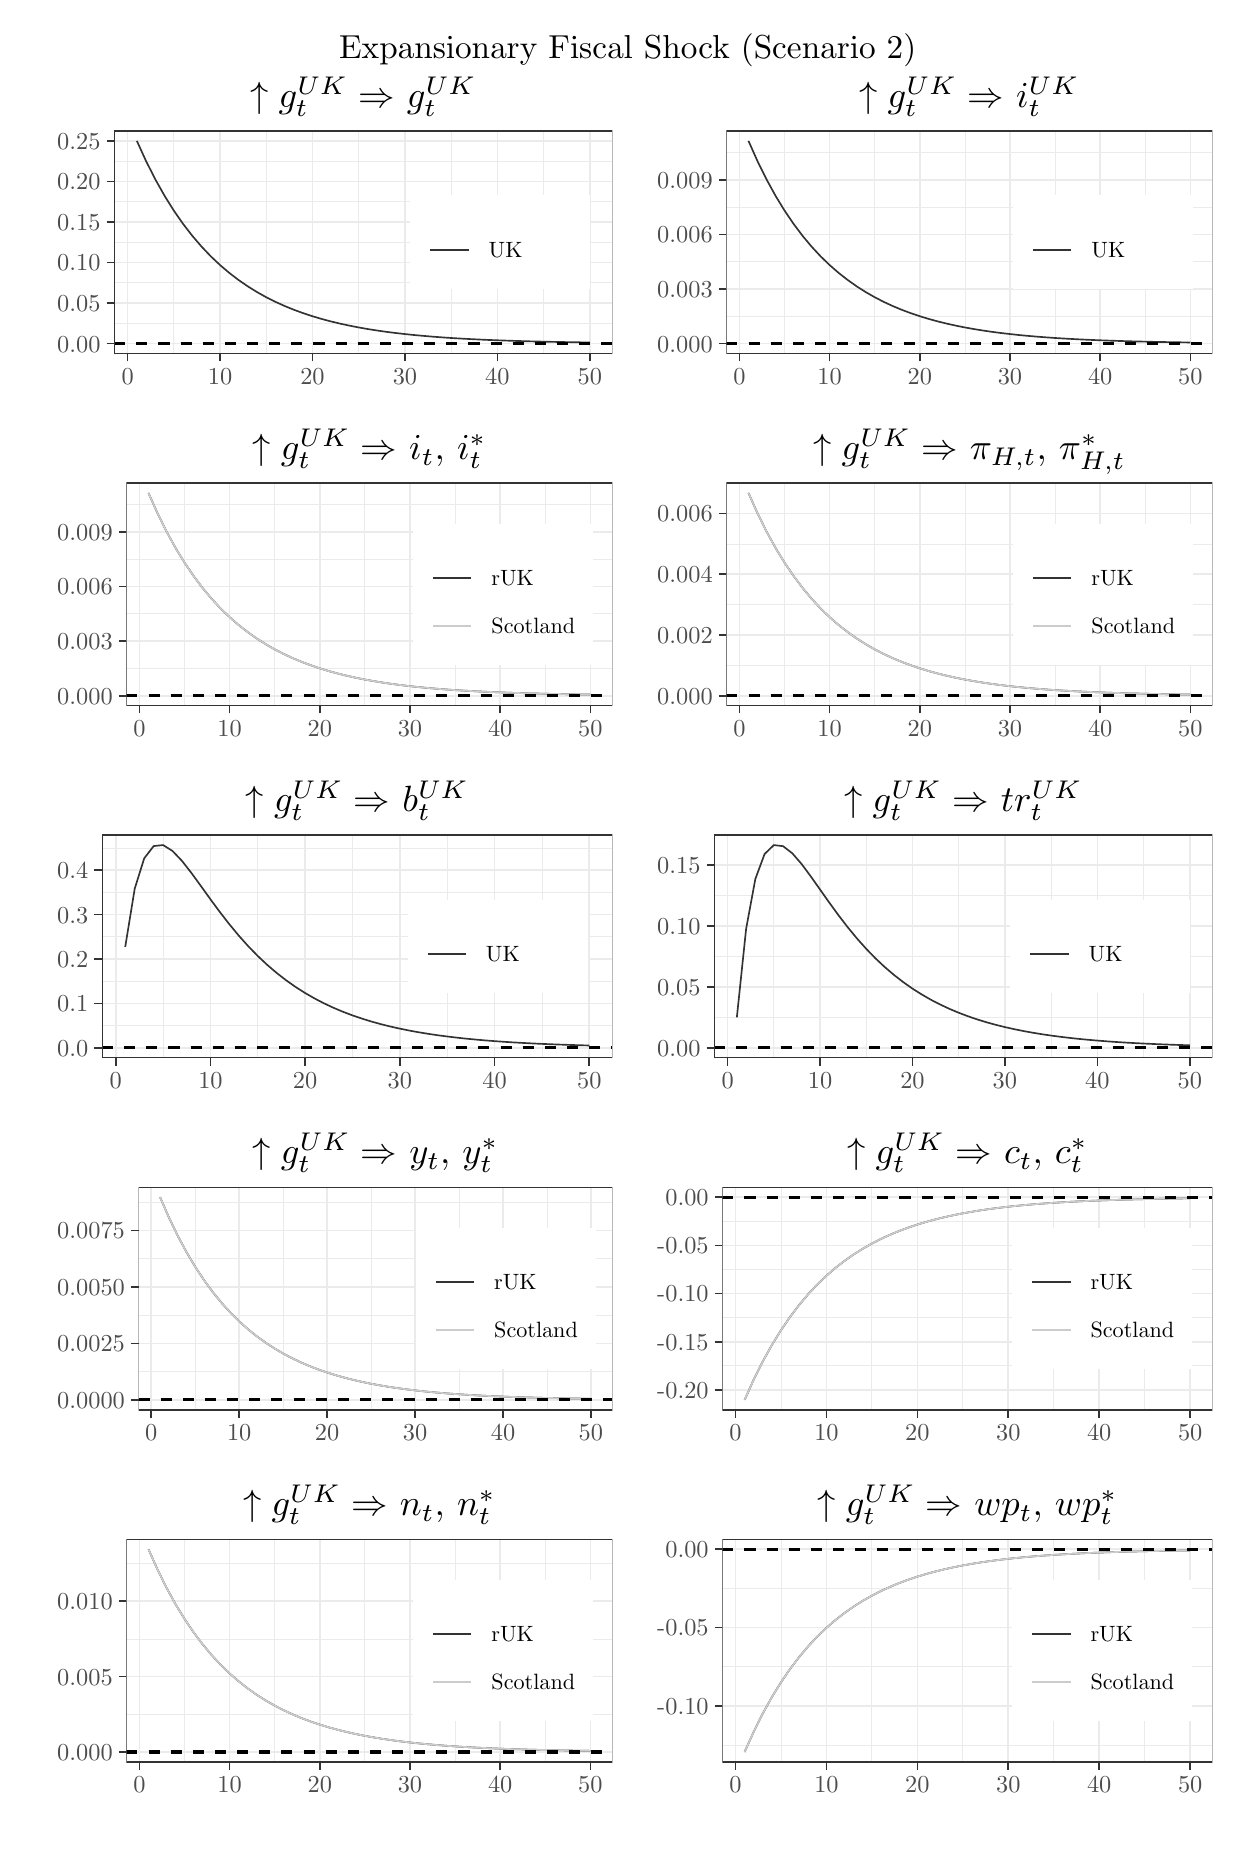
\begin{tikzpicture}[x=1pt,y=1pt]
\definecolor{fillColor}{RGB}{255,255,255}
\path[use as bounding box,fill=fillColor,fill opacity=0.00] (0,0) rectangle (433.62,650.43);
\begin{scope}
\path[clip] (  0.00,508.91) rectangle (216.81,636.14);
\definecolor{drawColor}{RGB}{255,255,255}
\definecolor{fillColor}{RGB}{255,255,255}

\path[draw=drawColor,line width= 0.6pt,line join=round,line cap=round,fill=fillColor] (  0.00,508.91) rectangle (216.81,636.14);
\end{scope}
\begin{scope}
\path[clip] ( 31.27,532.59) rectangle (211.31,613.18);
\definecolor{fillColor}{RGB}{255,255,255}

\path[fill=fillColor] ( 31.27,532.59) rectangle (211.31,613.18);
\definecolor{drawColor}{gray}{0.92}

\path[draw=drawColor,line width= 0.3pt,line join=round] ( 31.27,543.58) --
	(211.31,543.58);

\path[draw=drawColor,line width= 0.3pt,line join=round] ( 31.27,558.23) --
	(211.31,558.23);

\path[draw=drawColor,line width= 0.3pt,line join=round] ( 31.27,572.89) --
	(211.31,572.89);

\path[draw=drawColor,line width= 0.3pt,line join=round] ( 31.27,587.54) --
	(211.31,587.54);

\path[draw=drawColor,line width= 0.3pt,line join=round] ( 31.27,602.19) --
	(211.31,602.19);

\path[draw=drawColor,line width= 0.3pt,line join=round] ( 52.81,532.59) --
	( 52.81,613.18);

\path[draw=drawColor,line width= 0.3pt,line join=round] ( 86.22,532.59) --
	( 86.22,613.18);

\path[draw=drawColor,line width= 0.3pt,line join=round] (119.62,532.59) --
	(119.62,613.18);

\path[draw=drawColor,line width= 0.3pt,line join=round] (153.02,532.59) --
	(153.02,613.18);

\path[draw=drawColor,line width= 0.3pt,line join=round] (186.43,532.59) --
	(186.43,613.18);

\path[draw=drawColor,line width= 0.6pt,line join=round] ( 31.27,536.25) --
	(211.31,536.25);

\path[draw=drawColor,line width= 0.6pt,line join=round] ( 31.27,550.91) --
	(211.31,550.91);

\path[draw=drawColor,line width= 0.6pt,line join=round] ( 31.27,565.56) --
	(211.31,565.56);

\path[draw=drawColor,line width= 0.6pt,line join=round] ( 31.27,580.21) --
	(211.31,580.21);

\path[draw=drawColor,line width= 0.6pt,line join=round] ( 31.27,594.87) --
	(211.31,594.87);

\path[draw=drawColor,line width= 0.6pt,line join=round] ( 31.27,609.52) --
	(211.31,609.52);

\path[draw=drawColor,line width= 0.6pt,line join=round] ( 36.11,532.59) --
	( 36.11,613.18);

\path[draw=drawColor,line width= 0.6pt,line join=round] ( 69.52,532.59) --
	( 69.52,613.18);

\path[draw=drawColor,line width= 0.6pt,line join=round] (102.92,532.59) --
	(102.92,613.18);

\path[draw=drawColor,line width= 0.6pt,line join=round] (136.32,532.59) --
	(136.32,613.18);

\path[draw=drawColor,line width= 0.6pt,line join=round] (169.72,532.59) --
	(169.72,613.18);

\path[draw=drawColor,line width= 0.6pt,line join=round] (203.13,532.59) --
	(203.13,613.18);
\definecolor{drawColor}{gray}{0.20}

\path[draw=drawColor,line width= 0.6pt,line join=round] ( 39.45,609.52) --
	( 42.79,602.19) --
	( 46.13,595.60) --
	( 49.47,589.66) --
	( 52.81,584.32) --
	( 56.15,579.52) --
	( 59.50,575.19) --
	( 62.84,571.30) --
	( 66.18,567.79) --
	( 69.52,564.64) --
	( 72.86,561.80) --
	( 76.20,559.25) --
	( 79.54,556.95) --
	( 82.88,554.88) --
	( 86.22,553.01) --
	( 89.56,551.34) --
	( 92.90,549.83) --
	( 96.24,548.47) --
	( 99.58,547.25) --
	(102.92,546.15) --
	(106.26,545.16) --
	(109.60,544.27) --
	(112.94,543.47) --
	(116.28,542.75) --
	(119.62,542.10) --
	(122.96,541.51) --
	(126.30,540.99) --
	(129.64,540.51) --
	(132.98,540.09) --
	(136.32,539.71) --
	(139.66,539.36) --
	(143.00,539.05) --
	(146.34,538.77) --
	(149.68,538.52) --
	(153.02,538.29) --
	(156.36,538.09) --
	(159.70,537.91) --
	(163.04,537.74) --
	(166.38,537.59) --
	(169.72,537.46) --
	(173.06,537.34) --
	(176.40,537.23) --
	(179.74,537.13) --
	(183.08,537.04) --
	(186.43,536.97) --
	(189.77,536.89) --
	(193.11,536.83) --
	(196.45,536.77) --
	(199.79,536.72) --
	(203.13,536.67);
\definecolor{drawColor}{RGB}{0,0,0}

\path[draw=drawColor,line width= 1.1pt,dash pattern=on 4pt off 4pt ,line join=round] ( 31.27,536.25) -- (211.31,536.25);
\definecolor{drawColor}{gray}{0.20}

\path[draw=drawColor,line width= 0.6pt,line join=round,line cap=round] ( 31.27,532.59) rectangle (211.31,613.18);
\end{scope}
\begin{scope}
\path[clip] (  0.00,  0.00) rectangle (433.62,650.43);
\definecolor{drawColor}{gray}{0.30}

\node[text=drawColor,anchor=base east,inner sep=0pt, outer sep=0pt, scale=  0.88] at ( 26.32,533.22) {0.00};

\node[text=drawColor,anchor=base east,inner sep=0pt, outer sep=0pt, scale=  0.88] at ( 26.32,547.88) {0.05};

\node[text=drawColor,anchor=base east,inner sep=0pt, outer sep=0pt, scale=  0.88] at ( 26.32,562.53) {0.10};

\node[text=drawColor,anchor=base east,inner sep=0pt, outer sep=0pt, scale=  0.88] at ( 26.32,577.18) {0.15};

\node[text=drawColor,anchor=base east,inner sep=0pt, outer sep=0pt, scale=  0.88] at ( 26.32,591.83) {0.20};

\node[text=drawColor,anchor=base east,inner sep=0pt, outer sep=0pt, scale=  0.88] at ( 26.32,606.49) {0.25};
\end{scope}
\begin{scope}
\path[clip] (  0.00,  0.00) rectangle (433.62,650.43);
\definecolor{drawColor}{gray}{0.20}

\path[draw=drawColor,line width= 0.6pt,line join=round] ( 28.52,536.25) --
	( 31.27,536.25);

\path[draw=drawColor,line width= 0.6pt,line join=round] ( 28.52,550.91) --
	( 31.27,550.91);

\path[draw=drawColor,line width= 0.6pt,line join=round] ( 28.52,565.56) --
	( 31.27,565.56);

\path[draw=drawColor,line width= 0.6pt,line join=round] ( 28.52,580.21) --
	( 31.27,580.21);

\path[draw=drawColor,line width= 0.6pt,line join=round] ( 28.52,594.87) --
	( 31.27,594.87);

\path[draw=drawColor,line width= 0.6pt,line join=round] ( 28.52,609.52) --
	( 31.27,609.52);
\end{scope}
\begin{scope}
\path[clip] (  0.00,  0.00) rectangle (433.62,650.43);
\definecolor{drawColor}{gray}{0.20}

\path[draw=drawColor,line width= 0.6pt,line join=round] ( 36.11,529.84) --
	( 36.11,532.59);

\path[draw=drawColor,line width= 0.6pt,line join=round] ( 69.52,529.84) --
	( 69.52,532.59);

\path[draw=drawColor,line width= 0.6pt,line join=round] (102.92,529.84) --
	(102.92,532.59);

\path[draw=drawColor,line width= 0.6pt,line join=round] (136.32,529.84) --
	(136.32,532.59);

\path[draw=drawColor,line width= 0.6pt,line join=round] (169.72,529.84) --
	(169.72,532.59);

\path[draw=drawColor,line width= 0.6pt,line join=round] (203.13,529.84) --
	(203.13,532.59);
\end{scope}
\begin{scope}
\path[clip] (  0.00,  0.00) rectangle (433.62,650.43);
\definecolor{drawColor}{gray}{0.30}

\node[text=drawColor,anchor=base,inner sep=0pt, outer sep=0pt, scale=  0.88] at ( 36.11,521.58) {0};

\node[text=drawColor,anchor=base,inner sep=0pt, outer sep=0pt, scale=  0.88] at ( 69.52,521.58) {10};

\node[text=drawColor,anchor=base,inner sep=0pt, outer sep=0pt, scale=  0.88] at (102.92,521.58) {20};

\node[text=drawColor,anchor=base,inner sep=0pt, outer sep=0pt, scale=  0.88] at (136.32,521.58) {30};

\node[text=drawColor,anchor=base,inner sep=0pt, outer sep=0pt, scale=  0.88] at (169.72,521.58) {40};

\node[text=drawColor,anchor=base,inner sep=0pt, outer sep=0pt, scale=  0.88] at (203.13,521.58) {50};
\end{scope}
\begin{scope}
\path[clip] (  0.00,  0.00) rectangle (433.62,650.43);
\definecolor{fillColor}{RGB}{255,255,255}

\path[fill=fillColor] (138.26,555.96) rectangle (203.35,589.81);
\end{scope}
\begin{scope}
\path[clip] (  0.00,  0.00) rectangle (433.62,650.43);
\definecolor{fillColor}{RGB}{255,255,255}

\path[fill=fillColor] (143.76,561.46) rectangle (161.10,578.81);
\end{scope}
\begin{scope}
\path[clip] (  0.00,  0.00) rectangle (433.62,650.43);
\definecolor{drawColor}{gray}{0.20}

\path[draw=drawColor,line width= 0.6pt,line join=round] (145.49,570.14) -- (159.37,570.14);
\end{scope}
\begin{scope}
\path[clip] (  0.00,  0.00) rectangle (433.62,650.43);
\definecolor{drawColor}{RGB}{0,0,0}

\node[text=drawColor,anchor=base west,inner sep=0pt, outer sep=0pt, scale=  0.80] at (166.60,567.38) {UK};
\end{scope}
\begin{scope}
\path[clip] (  0.00,  0.00) rectangle (433.62,650.43);
\definecolor{drawColor}{RGB}{0,0,0}

\node[text=drawColor,anchor=base,inner sep=0pt, outer sep=0pt, scale=  1.32] at (121.29,621.55) {$\uparrow  g^{UK}_t \Rightarrow $ ${g^{UK}_t}$};
\end{scope}
\begin{scope}
\path[clip] (216.81,508.91) rectangle (433.62,636.14);
\definecolor{drawColor}{RGB}{255,255,255}
\definecolor{fillColor}{RGB}{255,255,255}

\path[draw=drawColor,line width= 0.6pt,line join=round,line cap=round,fill=fillColor] (216.81,508.91) rectangle (433.62,636.14);
\end{scope}
\begin{scope}
\path[clip] (252.48,532.59) rectangle (428.12,613.18);
\definecolor{fillColor}{RGB}{255,255,255}

\path[fill=fillColor] (252.48,532.59) rectangle (428.12,613.18);
\definecolor{drawColor}{gray}{0.92}

\path[draw=drawColor,line width= 0.3pt,line join=round] (252.48,546.12) --
	(428.12,546.12);

\path[draw=drawColor,line width= 0.3pt,line join=round] (252.48,565.85) --
	(428.12,565.85);

\path[draw=drawColor,line width= 0.3pt,line join=round] (252.48,585.58) --
	(428.12,585.58);

\path[draw=drawColor,line width= 0.3pt,line join=round] (252.48,605.31) --
	(428.12,605.31);

\path[draw=drawColor,line width= 0.3pt,line join=round] (273.50,532.59) --
	(273.50,613.18);

\path[draw=drawColor,line width= 0.3pt,line join=round] (306.08,532.59) --
	(306.08,613.18);

\path[draw=drawColor,line width= 0.3pt,line join=round] (338.67,532.59) --
	(338.67,613.18);

\path[draw=drawColor,line width= 0.3pt,line join=round] (371.26,532.59) --
	(371.26,613.18);

\path[draw=drawColor,line width= 0.3pt,line join=round] (403.84,532.59) --
	(403.84,613.18);

\path[draw=drawColor,line width= 0.6pt,line join=round] (252.48,536.25) --
	(428.12,536.25);

\path[draw=drawColor,line width= 0.6pt,line join=round] (252.48,555.98) --
	(428.12,555.98);

\path[draw=drawColor,line width= 0.6pt,line join=round] (252.48,575.71) --
	(428.12,575.71);

\path[draw=drawColor,line width= 0.6pt,line join=round] (252.48,595.44) --
	(428.12,595.44);

\path[draw=drawColor,line width= 0.6pt,line join=round] (257.20,532.59) --
	(257.20,613.18);

\path[draw=drawColor,line width= 0.6pt,line join=round] (289.79,532.59) --
	(289.79,613.18);

\path[draw=drawColor,line width= 0.6pt,line join=round] (322.38,532.59) --
	(322.38,613.18);

\path[draw=drawColor,line width= 0.6pt,line join=round] (354.96,532.59) --
	(354.96,613.18);

\path[draw=drawColor,line width= 0.6pt,line join=round] (387.55,532.59) --
	(387.55,613.18);

\path[draw=drawColor,line width= 0.6pt,line join=round] (420.14,532.59) --
	(420.14,613.18);
\definecolor{drawColor}{gray}{0.20}

\path[draw=drawColor,line width= 0.6pt,line join=round] (260.46,609.52) --
	(263.72,602.19) --
	(266.98,595.60) --
	(270.24,589.66) --
	(273.50,584.32) --
	(276.76,579.52) --
	(280.01,575.19) --
	(283.27,571.30) --
	(286.53,567.79) --
	(289.79,564.64) --
	(293.05,561.80) --
	(296.31,559.25) --
	(299.57,556.95) --
	(302.82,554.88) --
	(306.08,553.02) --
	(309.34,551.34) --
	(312.60,549.83) --
	(315.86,548.47) --
	(319.12,547.25) --
	(322.38,546.15) --
	(325.64,545.16) --
	(328.89,544.27) --
	(332.15,543.47) --
	(335.41,542.75) --
	(338.67,542.10) --
	(341.93,541.51) --
	(345.19,540.99) --
	(348.45,540.51) --
	(351.70,540.09) --
	(354.96,539.71) --
	(358.22,539.36) --
	(361.48,539.05) --
	(364.74,538.77) --
	(368.00,538.52) --
	(371.26,538.29) --
	(374.52,538.09) --
	(377.77,537.91) --
	(381.03,537.74) --
	(384.29,537.59) --
	(387.55,537.46) --
	(390.81,537.34) --
	(394.07,537.23) --
	(397.33,537.13) --
	(400.58,537.04) --
	(403.84,536.97) --
	(407.10,536.89) --
	(410.36,536.83) --
	(413.62,536.77) --
	(416.88,536.72) --
	(420.14,536.67);
\definecolor{drawColor}{RGB}{0,0,0}

\path[draw=drawColor,line width= 1.1pt,dash pattern=on 4pt off 4pt ,line join=round] (252.48,536.25) -- (428.12,536.25);
\definecolor{drawColor}{gray}{0.20}

\path[draw=drawColor,line width= 0.6pt,line join=round,line cap=round] (252.48,532.59) rectangle (428.12,613.18);
\end{scope}
\begin{scope}
\path[clip] (  0.00,  0.00) rectangle (433.62,650.43);
\definecolor{drawColor}{gray}{0.30}

\node[text=drawColor,anchor=base east,inner sep=0pt, outer sep=0pt, scale=  0.88] at (247.53,533.22) {0.000};

\node[text=drawColor,anchor=base east,inner sep=0pt, outer sep=0pt, scale=  0.88] at (247.53,552.95) {0.003};

\node[text=drawColor,anchor=base east,inner sep=0pt, outer sep=0pt, scale=  0.88] at (247.53,572.68) {0.006};

\node[text=drawColor,anchor=base east,inner sep=0pt, outer sep=0pt, scale=  0.88] at (247.53,592.41) {0.009};
\end{scope}
\begin{scope}
\path[clip] (  0.00,  0.00) rectangle (433.62,650.43);
\definecolor{drawColor}{gray}{0.20}

\path[draw=drawColor,line width= 0.6pt,line join=round] (249.73,536.25) --
	(252.48,536.25);

\path[draw=drawColor,line width= 0.6pt,line join=round] (249.73,555.98) --
	(252.48,555.98);

\path[draw=drawColor,line width= 0.6pt,line join=round] (249.73,575.71) --
	(252.48,575.71);

\path[draw=drawColor,line width= 0.6pt,line join=round] (249.73,595.44) --
	(252.48,595.44);
\end{scope}
\begin{scope}
\path[clip] (  0.00,  0.00) rectangle (433.62,650.43);
\definecolor{drawColor}{gray}{0.20}

\path[draw=drawColor,line width= 0.6pt,line join=round] (257.20,529.84) --
	(257.20,532.59);

\path[draw=drawColor,line width= 0.6pt,line join=round] (289.79,529.84) --
	(289.79,532.59);

\path[draw=drawColor,line width= 0.6pt,line join=round] (322.38,529.84) --
	(322.38,532.59);

\path[draw=drawColor,line width= 0.6pt,line join=round] (354.96,529.84) --
	(354.96,532.59);

\path[draw=drawColor,line width= 0.6pt,line join=round] (387.55,529.84) --
	(387.55,532.59);

\path[draw=drawColor,line width= 0.6pt,line join=round] (420.14,529.84) --
	(420.14,532.59);
\end{scope}
\begin{scope}
\path[clip] (  0.00,  0.00) rectangle (433.62,650.43);
\definecolor{drawColor}{gray}{0.30}

\node[text=drawColor,anchor=base,inner sep=0pt, outer sep=0pt, scale=  0.88] at (257.20,521.58) {0};

\node[text=drawColor,anchor=base,inner sep=0pt, outer sep=0pt, scale=  0.88] at (289.79,521.58) {10};

\node[text=drawColor,anchor=base,inner sep=0pt, outer sep=0pt, scale=  0.88] at (322.38,521.58) {20};

\node[text=drawColor,anchor=base,inner sep=0pt, outer sep=0pt, scale=  0.88] at (354.96,521.58) {30};

\node[text=drawColor,anchor=base,inner sep=0pt, outer sep=0pt, scale=  0.88] at (387.55,521.58) {40};

\node[text=drawColor,anchor=base,inner sep=0pt, outer sep=0pt, scale=  0.88] at (420.14,521.58) {50};
\end{scope}
\begin{scope}
\path[clip] (  0.00,  0.00) rectangle (433.62,650.43);
\definecolor{fillColor}{RGB}{255,255,255}

\path[fill=fillColor] (356.06,555.96) rectangle (421.15,589.81);
\end{scope}
\begin{scope}
\path[clip] (  0.00,  0.00) rectangle (433.62,650.43);
\definecolor{fillColor}{RGB}{255,255,255}

\path[fill=fillColor] (361.56,561.46) rectangle (378.90,578.81);
\end{scope}
\begin{scope}
\path[clip] (  0.00,  0.00) rectangle (433.62,650.43);
\definecolor{drawColor}{gray}{0.20}

\path[draw=drawColor,line width= 0.6pt,line join=round] (363.29,570.14) -- (377.17,570.14);
\end{scope}
\begin{scope}
\path[clip] (  0.00,  0.00) rectangle (433.62,650.43);
\definecolor{drawColor}{RGB}{0,0,0}

\node[text=drawColor,anchor=base west,inner sep=0pt, outer sep=0pt, scale=  0.80] at (384.40,567.38) {UK};
\end{scope}
\begin{scope}
\path[clip] (  0.00,  0.00) rectangle (433.62,650.43);
\definecolor{drawColor}{RGB}{0,0,0}

\node[text=drawColor,anchor=base,inner sep=0pt, outer sep=0pt, scale=  1.32] at (340.30,621.55) {$\uparrow  g^{UK}_t \Rightarrow $ ${i^{UK}_t}$};
\end{scope}
\begin{scope}
\path[clip] (  0.00,381.69) rectangle (216.81,508.91);
\definecolor{drawColor}{RGB}{255,255,255}
\definecolor{fillColor}{RGB}{255,255,255}

\path[draw=drawColor,line width= 0.6pt,line join=round,line cap=round,fill=fillColor] (  0.00,381.69) rectangle (216.81,508.91);
\end{scope}
\begin{scope}
\path[clip] ( 35.67,405.36) rectangle (211.31,485.95);
\definecolor{fillColor}{RGB}{255,255,255}

\path[fill=fillColor] ( 35.67,405.36) rectangle (211.31,485.95);
\definecolor{drawColor}{gray}{0.92}

\path[draw=drawColor,line width= 0.3pt,line join=round] ( 35.67,418.89) --
	(211.31,418.89);

\path[draw=drawColor,line width= 0.3pt,line join=round] ( 35.67,438.62) --
	(211.31,438.62);

\path[draw=drawColor,line width= 0.3pt,line join=round] ( 35.67,458.35) --
	(211.31,458.35);

\path[draw=drawColor,line width= 0.3pt,line join=round] ( 35.67,478.08) --
	(211.31,478.08);

\path[draw=drawColor,line width= 0.3pt,line join=round] ( 56.69,405.36) --
	( 56.69,485.95);

\path[draw=drawColor,line width= 0.3pt,line join=round] ( 89.27,405.36) --
	( 89.27,485.95);

\path[draw=drawColor,line width= 0.3pt,line join=round] (121.86,405.36) --
	(121.86,485.95);

\path[draw=drawColor,line width= 0.3pt,line join=round] (154.45,405.36) --
	(154.45,485.95);

\path[draw=drawColor,line width= 0.3pt,line join=round] (187.03,405.36) --
	(187.03,485.95);

\path[draw=drawColor,line width= 0.6pt,line join=round] ( 35.67,409.03) --
	(211.31,409.03);

\path[draw=drawColor,line width= 0.6pt,line join=round] ( 35.67,428.76) --
	(211.31,428.76);

\path[draw=drawColor,line width= 0.6pt,line join=round] ( 35.67,448.49) --
	(211.31,448.49);

\path[draw=drawColor,line width= 0.6pt,line join=round] ( 35.67,468.22) --
	(211.31,468.22);

\path[draw=drawColor,line width= 0.6pt,line join=round] ( 40.39,405.36) --
	( 40.39,485.95);

\path[draw=drawColor,line width= 0.6pt,line join=round] ( 72.98,405.36) --
	( 72.98,485.95);

\path[draw=drawColor,line width= 0.6pt,line join=round] (105.57,405.36) --
	(105.57,485.95);

\path[draw=drawColor,line width= 0.6pt,line join=round] (138.15,405.36) --
	(138.15,485.95);

\path[draw=drawColor,line width= 0.6pt,line join=round] (170.74,405.36) --
	(170.74,485.95);

\path[draw=drawColor,line width= 0.6pt,line join=round] (203.33,405.36) --
	(203.33,485.95);
\definecolor{drawColor}{gray}{0.20}

\path[draw=drawColor,line width= 0.6pt,line join=round] ( 43.65,482.29) --
	( 46.91,474.96) --
	( 50.17,468.37) --
	( 53.43,462.44) --
	( 56.69,457.09) --
	( 59.95,452.29) --
	( 63.20,447.96) --
	( 66.46,444.07) --
	( 69.72,440.56) --
	( 72.98,437.41) --
	( 76.24,434.57) --
	( 79.50,432.02) --
	( 82.76,429.72) --
	( 86.01,427.65) --
	( 89.27,425.79) --
	( 92.53,424.11) --
	( 95.79,422.60) --
	( 99.05,421.24) --
	(102.31,420.02) --
	(105.57,418.92) --
	(108.83,417.93) --
	(112.08,417.04) --
	(115.34,416.24) --
	(118.60,415.52) --
	(121.86,414.87) --
	(125.12,414.29) --
	(128.38,413.76) --
	(131.64,413.29) --
	(134.89,412.86) --
	(138.15,412.48) --
	(141.41,412.13) --
	(144.67,411.82) --
	(147.93,411.54) --
	(151.19,411.29) --
	(154.45,411.06) --
	(157.71,410.86) --
	(160.96,410.68) --
	(164.22,410.51) --
	(167.48,410.36) --
	(170.74,410.23) --
	(174.00,410.11) --
	(177.26,410.00) --
	(180.52,409.90) --
	(183.77,409.82) --
	(187.03,409.74) --
	(190.29,409.67) --
	(193.55,409.60) --
	(196.81,409.54) --
	(200.07,409.49) --
	(203.33,409.45);
\definecolor{drawColor}{gray}{0.80}

\path[draw=drawColor,line width= 0.6pt,line join=round] ( 43.65,482.29) --
	( 46.91,474.96) --
	( 50.17,468.37) --
	( 53.43,462.44) --
	( 56.69,457.09) --
	( 59.95,452.29) --
	( 63.20,447.96) --
	( 66.46,444.07) --
	( 69.72,440.56) --
	( 72.98,437.41) --
	( 76.24,434.57) --
	( 79.50,432.02) --
	( 82.76,429.72) --
	( 86.01,427.65) --
	( 89.27,425.79) --
	( 92.53,424.11) --
	( 95.79,422.60) --
	( 99.05,421.24) --
	(102.31,420.02) --
	(105.57,418.92) --
	(108.83,417.93) --
	(112.08,417.04) --
	(115.34,416.24) --
	(118.60,415.52) --
	(121.86,414.87) --
	(125.12,414.29) --
	(128.38,413.76) --
	(131.64,413.29) --
	(134.89,412.86) --
	(138.15,412.48) --
	(141.41,412.13) --
	(144.67,411.82) --
	(147.93,411.54) --
	(151.19,411.29) --
	(154.45,411.06) --
	(157.71,410.86) --
	(160.96,410.68) --
	(164.22,410.51) --
	(167.48,410.36) --
	(170.74,410.23) --
	(174.00,410.11) --
	(177.26,410.00) --
	(180.52,409.90) --
	(183.77,409.82) --
	(187.03,409.74) --
	(190.29,409.67) --
	(193.55,409.60) --
	(196.81,409.54) --
	(200.07,409.49) --
	(203.33,409.45);
\definecolor{drawColor}{RGB}{0,0,0}

\path[draw=drawColor,line width= 1.1pt,dash pattern=on 4pt off 4pt ,line join=round] ( 35.67,409.03) -- (211.31,409.03);
\definecolor{drawColor}{gray}{0.20}

\path[draw=drawColor,line width= 0.6pt,line join=round,line cap=round] ( 35.67,405.36) rectangle (211.31,485.95);
\end{scope}
\begin{scope}
\path[clip] (  0.00,  0.00) rectangle (433.62,650.43);
\definecolor{drawColor}{gray}{0.30}

\node[text=drawColor,anchor=base east,inner sep=0pt, outer sep=0pt, scale=  0.88] at ( 30.72,406.00) {0.000};

\node[text=drawColor,anchor=base east,inner sep=0pt, outer sep=0pt, scale=  0.88] at ( 30.72,425.73) {0.003};

\node[text=drawColor,anchor=base east,inner sep=0pt, outer sep=0pt, scale=  0.88] at ( 30.72,445.46) {0.006};

\node[text=drawColor,anchor=base east,inner sep=0pt, outer sep=0pt, scale=  0.88] at ( 30.72,465.18) {0.009};
\end{scope}
\begin{scope}
\path[clip] (  0.00,  0.00) rectangle (433.62,650.43);
\definecolor{drawColor}{gray}{0.20}

\path[draw=drawColor,line width= 0.6pt,line join=round] ( 32.92,409.03) --
	( 35.67,409.03);

\path[draw=drawColor,line width= 0.6pt,line join=round] ( 32.92,428.76) --
	( 35.67,428.76);

\path[draw=drawColor,line width= 0.6pt,line join=round] ( 32.92,448.49) --
	( 35.67,448.49);

\path[draw=drawColor,line width= 0.6pt,line join=round] ( 32.92,468.22) --
	( 35.67,468.22);
\end{scope}
\begin{scope}
\path[clip] (  0.00,  0.00) rectangle (433.62,650.43);
\definecolor{drawColor}{gray}{0.20}

\path[draw=drawColor,line width= 0.6pt,line join=round] ( 40.39,402.61) --
	( 40.39,405.36);

\path[draw=drawColor,line width= 0.6pt,line join=round] ( 72.98,402.61) --
	( 72.98,405.36);

\path[draw=drawColor,line width= 0.6pt,line join=round] (105.57,402.61) --
	(105.57,405.36);

\path[draw=drawColor,line width= 0.6pt,line join=round] (138.15,402.61) --
	(138.15,405.36);

\path[draw=drawColor,line width= 0.6pt,line join=round] (170.74,402.61) --
	(170.74,405.36);

\path[draw=drawColor,line width= 0.6pt,line join=round] (203.33,402.61) --
	(203.33,405.36);
\end{scope}
\begin{scope}
\path[clip] (  0.00,  0.00) rectangle (433.62,650.43);
\definecolor{drawColor}{gray}{0.30}

\node[text=drawColor,anchor=base,inner sep=0pt, outer sep=0pt, scale=  0.88] at ( 40.39,394.35) {0};

\node[text=drawColor,anchor=base,inner sep=0pt, outer sep=0pt, scale=  0.88] at ( 72.98,394.35) {10};

\node[text=drawColor,anchor=base,inner sep=0pt, outer sep=0pt, scale=  0.88] at (105.57,394.35) {20};

\node[text=drawColor,anchor=base,inner sep=0pt, outer sep=0pt, scale=  0.88] at (138.15,394.35) {30};

\node[text=drawColor,anchor=base,inner sep=0pt, outer sep=0pt, scale=  0.88] at (170.74,394.35) {40};

\node[text=drawColor,anchor=base,inner sep=0pt, outer sep=0pt, scale=  0.88] at (203.33,394.35) {50};
\end{scope}
\begin{scope}
\path[clip] (  0.00,  0.00) rectangle (433.62,650.43);
\definecolor{fillColor}{RGB}{255,255,255}

\path[fill=fillColor] (139.25,420.06) rectangle (204.34,471.25);
\end{scope}
\begin{scope}
\path[clip] (  0.00,  0.00) rectangle (433.62,650.43);
\definecolor{fillColor}{RGB}{255,255,255}

\path[fill=fillColor] (144.75,442.91) rectangle (162.09,460.25);
\end{scope}
\begin{scope}
\path[clip] (  0.00,  0.00) rectangle (433.62,650.43);
\definecolor{drawColor}{gray}{0.20}

\path[draw=drawColor,line width= 0.6pt,line join=round] (146.48,451.58) -- (160.36,451.58);
\end{scope}
\begin{scope}
\path[clip] (  0.00,  0.00) rectangle (433.62,650.43);
\definecolor{fillColor}{RGB}{255,255,255}

\path[fill=fillColor] (144.75,425.56) rectangle (162.09,442.91);
\end{scope}
\begin{scope}
\path[clip] (  0.00,  0.00) rectangle (433.62,650.43);
\definecolor{drawColor}{gray}{0.80}

\path[draw=drawColor,line width= 0.6pt,line join=round] (146.48,434.24) -- (160.36,434.24);
\end{scope}
\begin{scope}
\path[clip] (  0.00,  0.00) rectangle (433.62,650.43);
\definecolor{drawColor}{RGB}{0,0,0}

\node[text=drawColor,anchor=base west,inner sep=0pt, outer sep=0pt, scale=  0.80] at (167.59,448.83) {rUK};
\end{scope}
\begin{scope}
\path[clip] (  0.00,  0.00) rectangle (433.62,650.43);
\definecolor{drawColor}{RGB}{0,0,0}

\node[text=drawColor,anchor=base west,inner sep=0pt, outer sep=0pt, scale=  0.80] at (167.59,431.48) {Scotland};
\end{scope}
\begin{scope}
\path[clip] (  0.00,  0.00) rectangle (433.62,650.43);
\definecolor{drawColor}{RGB}{0,0,0}

\node[text=drawColor,anchor=base,inner sep=0pt, outer sep=0pt, scale=  1.32] at (123.49,494.32) {$\uparrow  g^{UK}_t \Rightarrow $ ${i_t}$, ${i^*_t}$};
\end{scope}
\begin{scope}
\path[clip] (216.81,381.69) rectangle (433.62,508.91);
\definecolor{drawColor}{RGB}{255,255,255}
\definecolor{fillColor}{RGB}{255,255,255}

\path[draw=drawColor,line width= 0.6pt,line join=round,line cap=round,fill=fillColor] (216.81,381.69) rectangle (433.62,508.91);
\end{scope}
\begin{scope}
\path[clip] (252.48,405.36) rectangle (428.12,485.95);
\definecolor{fillColor}{RGB}{255,255,255}

\path[fill=fillColor] (252.48,405.36) rectangle (428.12,485.95);
\definecolor{drawColor}{gray}{0.92}

\path[draw=drawColor,line width= 0.3pt,line join=round] (252.48,420.00) --
	(428.12,420.00);

\path[draw=drawColor,line width= 0.3pt,line join=round] (252.48,441.93) --
	(428.12,441.93);

\path[draw=drawColor,line width= 0.3pt,line join=round] (252.48,463.87) --
	(428.12,463.87);

\path[draw=drawColor,line width= 0.3pt,line join=round] (252.48,485.81) --
	(428.12,485.81);

\path[draw=drawColor,line width= 0.3pt,line join=round] (273.50,405.36) --
	(273.50,485.95);

\path[draw=drawColor,line width= 0.3pt,line join=round] (306.08,405.36) --
	(306.08,485.95);

\path[draw=drawColor,line width= 0.3pt,line join=round] (338.67,405.36) --
	(338.67,485.95);

\path[draw=drawColor,line width= 0.3pt,line join=round] (371.26,405.36) --
	(371.26,485.95);

\path[draw=drawColor,line width= 0.3pt,line join=round] (403.84,405.36) --
	(403.84,485.95);

\path[draw=drawColor,line width= 0.6pt,line join=round] (252.48,409.03) --
	(428.12,409.03);

\path[draw=drawColor,line width= 0.6pt,line join=round] (252.48,430.96) --
	(428.12,430.96);

\path[draw=drawColor,line width= 0.6pt,line join=round] (252.48,452.90) --
	(428.12,452.90);

\path[draw=drawColor,line width= 0.6pt,line join=round] (252.48,474.84) --
	(428.12,474.84);

\path[draw=drawColor,line width= 0.6pt,line join=round] (257.20,405.36) --
	(257.20,485.95);

\path[draw=drawColor,line width= 0.6pt,line join=round] (289.79,405.36) --
	(289.79,485.95);

\path[draw=drawColor,line width= 0.6pt,line join=round] (322.38,405.36) --
	(322.38,485.95);

\path[draw=drawColor,line width= 0.6pt,line join=round] (354.96,405.36) --
	(354.96,485.95);

\path[draw=drawColor,line width= 0.6pt,line join=round] (387.55,405.36) --
	(387.55,485.95);

\path[draw=drawColor,line width= 0.6pt,line join=round] (420.14,405.36) --
	(420.14,485.95);
\definecolor{drawColor}{gray}{0.20}

\path[draw=drawColor,line width= 0.6pt,line join=round] (260.46,482.29) --
	(263.72,474.96) --
	(266.98,468.37) --
	(270.24,462.43) --
	(273.50,457.09) --
	(276.76,452.29) --
	(280.01,447.96) --
	(283.27,444.07) --
	(286.53,440.56) --
	(289.79,437.41) --
	(293.05,434.57) --
	(296.31,432.02) --
	(299.57,429.72) --
	(302.82,427.65) --
	(306.08,425.79) --
	(309.34,424.11) --
	(312.60,422.60) --
	(315.86,421.24) --
	(319.12,420.02) --
	(322.38,418.92) --
	(325.64,417.93) --
	(328.89,417.04) --
	(332.15,416.24) --
	(335.41,415.52) --
	(338.67,414.87) --
	(341.93,414.29) --
	(345.19,413.76) --
	(348.45,413.29) --
	(351.70,412.86) --
	(354.96,412.48) --
	(358.22,412.13) --
	(361.48,411.82) --
	(364.74,411.54) --
	(368.00,411.29) --
	(371.26,411.06) --
	(374.52,410.86) --
	(377.77,410.68) --
	(381.03,410.51) --
	(384.29,410.36) --
	(387.55,410.23) --
	(390.81,410.11) --
	(394.07,410.00) --
	(397.33,409.90) --
	(400.58,409.82) --
	(403.84,409.74) --
	(407.10,409.67) --
	(410.36,409.60) --
	(413.62,409.54) --
	(416.88,409.49) --
	(420.14,409.45);
\definecolor{drawColor}{gray}{0.80}

\path[draw=drawColor,line width= 0.6pt,line join=round] (260.46,482.29) --
	(263.72,474.96) --
	(266.98,468.37) --
	(270.24,462.43) --
	(273.50,457.09) --
	(276.76,452.29) --
	(280.01,447.96) --
	(283.27,444.07) --
	(286.53,440.56) --
	(289.79,437.41) --
	(293.05,434.57) --
	(296.31,432.02) --
	(299.57,429.72) --
	(302.82,427.65) --
	(306.08,425.79) --
	(309.34,424.11) --
	(312.60,422.60) --
	(315.86,421.24) --
	(319.12,420.02) --
	(322.38,418.92) --
	(325.64,417.93) --
	(328.89,417.04) --
	(332.15,416.24) --
	(335.41,415.52) --
	(338.67,414.87) --
	(341.93,414.29) --
	(345.19,413.76) --
	(348.45,413.29) --
	(351.70,412.86) --
	(354.96,412.48) --
	(358.22,412.13) --
	(361.48,411.82) --
	(364.74,411.54) --
	(368.00,411.29) --
	(371.26,411.06) --
	(374.52,410.86) --
	(377.77,410.68) --
	(381.03,410.51) --
	(384.29,410.36) --
	(387.55,410.23) --
	(390.81,410.11) --
	(394.07,410.00) --
	(397.33,409.90) --
	(400.58,409.82) --
	(403.84,409.74) --
	(407.10,409.67) --
	(410.36,409.60) --
	(413.62,409.54) --
	(416.88,409.49) --
	(420.14,409.45);
\definecolor{drawColor}{RGB}{0,0,0}

\path[draw=drawColor,line width= 1.1pt,dash pattern=on 4pt off 4pt ,line join=round] (252.48,409.03) -- (428.12,409.03);
\definecolor{drawColor}{gray}{0.20}

\path[draw=drawColor,line width= 0.6pt,line join=round,line cap=round] (252.48,405.36) rectangle (428.12,485.95);
\end{scope}
\begin{scope}
\path[clip] (  0.00,  0.00) rectangle (433.62,650.43);
\definecolor{drawColor}{gray}{0.30}

\node[text=drawColor,anchor=base east,inner sep=0pt, outer sep=0pt, scale=  0.88] at (247.53,406.00) {0.000};

\node[text=drawColor,anchor=base east,inner sep=0pt, outer sep=0pt, scale=  0.88] at (247.53,427.93) {0.002};

\node[text=drawColor,anchor=base east,inner sep=0pt, outer sep=0pt, scale=  0.88] at (247.53,449.87) {0.004};

\node[text=drawColor,anchor=base east,inner sep=0pt, outer sep=0pt, scale=  0.88] at (247.53,471.81) {0.006};
\end{scope}
\begin{scope}
\path[clip] (  0.00,  0.00) rectangle (433.62,650.43);
\definecolor{drawColor}{gray}{0.20}

\path[draw=drawColor,line width= 0.6pt,line join=round] (249.73,409.03) --
	(252.48,409.03);

\path[draw=drawColor,line width= 0.6pt,line join=round] (249.73,430.96) --
	(252.48,430.96);

\path[draw=drawColor,line width= 0.6pt,line join=round] (249.73,452.90) --
	(252.48,452.90);

\path[draw=drawColor,line width= 0.6pt,line join=round] (249.73,474.84) --
	(252.48,474.84);
\end{scope}
\begin{scope}
\path[clip] (  0.00,  0.00) rectangle (433.62,650.43);
\definecolor{drawColor}{gray}{0.20}

\path[draw=drawColor,line width= 0.6pt,line join=round] (257.20,402.61) --
	(257.20,405.36);

\path[draw=drawColor,line width= 0.6pt,line join=round] (289.79,402.61) --
	(289.79,405.36);

\path[draw=drawColor,line width= 0.6pt,line join=round] (322.38,402.61) --
	(322.38,405.36);

\path[draw=drawColor,line width= 0.6pt,line join=round] (354.96,402.61) --
	(354.96,405.36);

\path[draw=drawColor,line width= 0.6pt,line join=round] (387.55,402.61) --
	(387.55,405.36);

\path[draw=drawColor,line width= 0.6pt,line join=round] (420.14,402.61) --
	(420.14,405.36);
\end{scope}
\begin{scope}
\path[clip] (  0.00,  0.00) rectangle (433.62,650.43);
\definecolor{drawColor}{gray}{0.30}

\node[text=drawColor,anchor=base,inner sep=0pt, outer sep=0pt, scale=  0.88] at (257.20,394.35) {0};

\node[text=drawColor,anchor=base,inner sep=0pt, outer sep=0pt, scale=  0.88] at (289.79,394.35) {10};

\node[text=drawColor,anchor=base,inner sep=0pt, outer sep=0pt, scale=  0.88] at (322.38,394.35) {20};

\node[text=drawColor,anchor=base,inner sep=0pt, outer sep=0pt, scale=  0.88] at (354.96,394.35) {30};

\node[text=drawColor,anchor=base,inner sep=0pt, outer sep=0pt, scale=  0.88] at (387.55,394.35) {40};

\node[text=drawColor,anchor=base,inner sep=0pt, outer sep=0pt, scale=  0.88] at (420.14,394.35) {50};
\end{scope}
\begin{scope}
\path[clip] (  0.00,  0.00) rectangle (433.62,650.43);
\definecolor{fillColor}{RGB}{255,255,255}

\path[fill=fillColor] (356.06,420.06) rectangle (421.15,471.25);
\end{scope}
\begin{scope}
\path[clip] (  0.00,  0.00) rectangle (433.62,650.43);
\definecolor{fillColor}{RGB}{255,255,255}

\path[fill=fillColor] (361.56,442.91) rectangle (378.90,460.25);
\end{scope}
\begin{scope}
\path[clip] (  0.00,  0.00) rectangle (433.62,650.43);
\definecolor{drawColor}{gray}{0.20}

\path[draw=drawColor,line width= 0.6pt,line join=round] (363.29,451.58) -- (377.17,451.58);
\end{scope}
\begin{scope}
\path[clip] (  0.00,  0.00) rectangle (433.62,650.43);
\definecolor{fillColor}{RGB}{255,255,255}

\path[fill=fillColor] (361.56,425.56) rectangle (378.90,442.91);
\end{scope}
\begin{scope}
\path[clip] (  0.00,  0.00) rectangle (433.62,650.43);
\definecolor{drawColor}{gray}{0.80}

\path[draw=drawColor,line width= 0.6pt,line join=round] (363.29,434.24) -- (377.17,434.24);
\end{scope}
\begin{scope}
\path[clip] (  0.00,  0.00) rectangle (433.62,650.43);
\definecolor{drawColor}{RGB}{0,0,0}

\node[text=drawColor,anchor=base west,inner sep=0pt, outer sep=0pt, scale=  0.80] at (384.40,448.83) {rUK};
\end{scope}
\begin{scope}
\path[clip] (  0.00,  0.00) rectangle (433.62,650.43);
\definecolor{drawColor}{RGB}{0,0,0}

\node[text=drawColor,anchor=base west,inner sep=0pt, outer sep=0pt, scale=  0.80] at (384.40,431.48) {Scotland};
\end{scope}
\begin{scope}
\path[clip] (  0.00,  0.00) rectangle (433.62,650.43);
\definecolor{drawColor}{RGB}{0,0,0}

\node[text=drawColor,anchor=base,inner sep=0pt, outer sep=0pt, scale=  1.32] at (340.30,494.32) {$\uparrow  g^{UK}_t \Rightarrow $ ${\pi_{H,t}}$, ${\pi^*_{H,t}}$};
\end{scope}
\begin{scope}
\path[clip] (  0.00,254.46) rectangle (216.81,381.69);
\definecolor{drawColor}{RGB}{255,255,255}
\definecolor{fillColor}{RGB}{255,255,255}

\path[draw=drawColor,line width= 0.6pt,line join=round,line cap=round,fill=fillColor] (  0.00,254.46) rectangle (216.81,381.69);
\end{scope}
\begin{scope}
\path[clip] ( 26.87,278.13) rectangle (211.31,358.72);
\definecolor{fillColor}{RGB}{255,255,255}

\path[fill=fillColor] ( 26.87,278.13) rectangle (211.31,358.72);
\definecolor{drawColor}{gray}{0.92}

\path[draw=drawColor,line width= 0.3pt,line join=round] ( 26.87,289.82) --
	(211.31,289.82);

\path[draw=drawColor,line width= 0.3pt,line join=round] ( 26.87,305.86) --
	(211.31,305.86);

\path[draw=drawColor,line width= 0.3pt,line join=round] ( 26.87,321.91) --
	(211.31,321.91);

\path[draw=drawColor,line width= 0.3pt,line join=round] ( 26.87,337.95) --
	(211.31,337.95);

\path[draw=drawColor,line width= 0.3pt,line join=round] ( 26.87,354.00) --
	(211.31,354.00);

\path[draw=drawColor,line width= 0.3pt,line join=round] ( 48.94,278.13) --
	( 48.94,358.72);

\path[draw=drawColor,line width= 0.3pt,line join=round] ( 83.16,278.13) --
	( 83.16,358.72);

\path[draw=drawColor,line width= 0.3pt,line join=round] (117.38,278.13) --
	(117.38,358.72);

\path[draw=drawColor,line width= 0.3pt,line join=round] (151.60,278.13) --
	(151.60,358.72);

\path[draw=drawColor,line width= 0.3pt,line join=round] (185.82,278.13) --
	(185.82,358.72);

\path[draw=drawColor,line width= 0.6pt,line join=round] ( 26.87,281.80) --
	(211.31,281.80);

\path[draw=drawColor,line width= 0.6pt,line join=round] ( 26.87,297.84) --
	(211.31,297.84);

\path[draw=drawColor,line width= 0.6pt,line join=round] ( 26.87,313.89) --
	(211.31,313.89);

\path[draw=drawColor,line width= 0.6pt,line join=round] ( 26.87,329.93) --
	(211.31,329.93);

\path[draw=drawColor,line width= 0.6pt,line join=round] ( 26.87,345.97) --
	(211.31,345.97);

\path[draw=drawColor,line width= 0.6pt,line join=round] ( 31.83,278.13) --
	( 31.83,358.72);

\path[draw=drawColor,line width= 0.6pt,line join=round] ( 66.05,278.13) --
	( 66.05,358.72);

\path[draw=drawColor,line width= 0.6pt,line join=round] (100.27,278.13) --
	(100.27,358.72);

\path[draw=drawColor,line width= 0.6pt,line join=round] (134.49,278.13) --
	(134.49,358.72);

\path[draw=drawColor,line width= 0.6pt,line join=round] (168.71,278.13) --
	(168.71,358.72);

\path[draw=drawColor,line width= 0.6pt,line join=round] (202.93,278.13) --
	(202.93,358.72);
\definecolor{drawColor}{gray}{0.20}

\path[draw=drawColor,line width= 0.6pt,line join=round] ( 35.25,318.26) --
	( 38.68,339.29) --
	( 42.10,350.24) --
	( 45.52,354.70) --
	( 48.94,355.06) --
	( 52.36,352.91) --
	( 55.79,349.30) --
	( 59.21,344.92) --
	( 62.63,340.22) --
	( 66.05,335.46) --
	( 69.47,330.83) --
	( 72.90,326.42) --
	( 76.32,322.30) --
	( 79.74,318.47) --
	( 83.16,314.96) --
	( 86.58,311.75) --
	( 90.00,308.83) --
	( 93.43,306.17) --
	( 96.85,303.76) --
	(100.27,301.59) --
	(103.69,299.63) --
	(107.11,297.85) --
	(110.54,296.25) --
	(113.96,294.81) --
	(117.38,293.51) --
	(120.80,292.35) --
	(124.22,291.29) --
	(127.65,290.34) --
	(131.07,289.49) --
	(134.49,288.72) --
	(137.91,288.03) --
	(141.33,287.41) --
	(144.75,286.85) --
	(148.18,286.34) --
	(151.60,285.89) --
	(155.02,285.48) --
	(158.44,285.11) --
	(161.86,284.78) --
	(165.29,284.48) --
	(168.71,284.21) --
	(172.13,283.97) --
	(175.55,283.75) --
	(178.97,283.56) --
	(182.40,283.38) --
	(185.82,283.22) --
	(189.24,283.08) --
	(192.66,282.95) --
	(196.08,282.84) --
	(199.50,282.73) --
	(202.93,282.64);
\definecolor{drawColor}{RGB}{0,0,0}

\path[draw=drawColor,line width= 1.1pt,dash pattern=on 4pt off 4pt ,line join=round] ( 26.87,281.80) -- (211.31,281.80);
\definecolor{drawColor}{gray}{0.20}

\path[draw=drawColor,line width= 0.6pt,line join=round,line cap=round] ( 26.87,278.13) rectangle (211.31,358.72);
\end{scope}
\begin{scope}
\path[clip] (  0.00,  0.00) rectangle (433.62,650.43);
\definecolor{drawColor}{gray}{0.30}

\node[text=drawColor,anchor=base east,inner sep=0pt, outer sep=0pt, scale=  0.88] at ( 21.92,278.77) {0.0};

\node[text=drawColor,anchor=base east,inner sep=0pt, outer sep=0pt, scale=  0.88] at ( 21.92,294.81) {0.1};

\node[text=drawColor,anchor=base east,inner sep=0pt, outer sep=0pt, scale=  0.88] at ( 21.92,310.86) {0.2};

\node[text=drawColor,anchor=base east,inner sep=0pt, outer sep=0pt, scale=  0.88] at ( 21.92,326.90) {0.3};

\node[text=drawColor,anchor=base east,inner sep=0pt, outer sep=0pt, scale=  0.88] at ( 21.92,342.94) {0.4};
\end{scope}
\begin{scope}
\path[clip] (  0.00,  0.00) rectangle (433.62,650.43);
\definecolor{drawColor}{gray}{0.20}

\path[draw=drawColor,line width= 0.6pt,line join=round] ( 24.12,281.80) --
	( 26.87,281.80);

\path[draw=drawColor,line width= 0.6pt,line join=round] ( 24.12,297.84) --
	( 26.87,297.84);

\path[draw=drawColor,line width= 0.6pt,line join=round] ( 24.12,313.89) --
	( 26.87,313.89);

\path[draw=drawColor,line width= 0.6pt,line join=round] ( 24.12,329.93) --
	( 26.87,329.93);

\path[draw=drawColor,line width= 0.6pt,line join=round] ( 24.12,345.97) --
	( 26.87,345.97);
\end{scope}
\begin{scope}
\path[clip] (  0.00,  0.00) rectangle (433.62,650.43);
\definecolor{drawColor}{gray}{0.20}

\path[draw=drawColor,line width= 0.6pt,line join=round] ( 31.83,275.38) --
	( 31.83,278.13);

\path[draw=drawColor,line width= 0.6pt,line join=round] ( 66.05,275.38) --
	( 66.05,278.13);

\path[draw=drawColor,line width= 0.6pt,line join=round] (100.27,275.38) --
	(100.27,278.13);

\path[draw=drawColor,line width= 0.6pt,line join=round] (134.49,275.38) --
	(134.49,278.13);

\path[draw=drawColor,line width= 0.6pt,line join=round] (168.71,275.38) --
	(168.71,278.13);

\path[draw=drawColor,line width= 0.6pt,line join=round] (202.93,275.38) --
	(202.93,278.13);
\end{scope}
\begin{scope}
\path[clip] (  0.00,  0.00) rectangle (433.62,650.43);
\definecolor{drawColor}{gray}{0.30}

\node[text=drawColor,anchor=base,inner sep=0pt, outer sep=0pt, scale=  0.88] at ( 31.83,267.12) {0};

\node[text=drawColor,anchor=base,inner sep=0pt, outer sep=0pt, scale=  0.88] at ( 66.05,267.12) {10};

\node[text=drawColor,anchor=base,inner sep=0pt, outer sep=0pt, scale=  0.88] at (100.27,267.12) {20};

\node[text=drawColor,anchor=base,inner sep=0pt, outer sep=0pt, scale=  0.88] at (134.49,267.12) {30};

\node[text=drawColor,anchor=base,inner sep=0pt, outer sep=0pt, scale=  0.88] at (168.71,267.12) {40};

\node[text=drawColor,anchor=base,inner sep=0pt, outer sep=0pt, scale=  0.88] at (202.93,267.12) {50};
\end{scope}
\begin{scope}
\path[clip] (  0.00,  0.00) rectangle (433.62,650.43);
\definecolor{fillColor}{RGB}{255,255,255}

\path[fill=fillColor] (137.27,301.51) rectangle (202.36,335.35);
\end{scope}
\begin{scope}
\path[clip] (  0.00,  0.00) rectangle (433.62,650.43);
\definecolor{fillColor}{RGB}{255,255,255}

\path[fill=fillColor] (142.77,307.01) rectangle (160.11,324.35);
\end{scope}
\begin{scope}
\path[clip] (  0.00,  0.00) rectangle (433.62,650.43);
\definecolor{drawColor}{gray}{0.20}

\path[draw=drawColor,line width= 0.6pt,line join=round] (144.50,315.68) -- (158.38,315.68);
\end{scope}
\begin{scope}
\path[clip] (  0.00,  0.00) rectangle (433.62,650.43);
\definecolor{drawColor}{RGB}{0,0,0}

\node[text=drawColor,anchor=base west,inner sep=0pt, outer sep=0pt, scale=  0.80] at (165.61,312.92) {UK};
\end{scope}
\begin{scope}
\path[clip] (  0.00,  0.00) rectangle (433.62,650.43);
\definecolor{drawColor}{RGB}{0,0,0}

\node[text=drawColor,anchor=base,inner sep=0pt, outer sep=0pt, scale=  1.32] at (119.09,367.09) {$\uparrow  g^{UK}_t \Rightarrow $ ${b^{UK}_t}$};
\end{scope}
\begin{scope}
\path[clip] (216.81,254.46) rectangle (433.62,381.69);
\definecolor{drawColor}{RGB}{255,255,255}
\definecolor{fillColor}{RGB}{255,255,255}

\path[draw=drawColor,line width= 0.6pt,line join=round,line cap=round,fill=fillColor] (216.81,254.46) rectangle (433.62,381.69);
\end{scope}
\begin{scope}
\path[clip] (248.08,278.13) rectangle (428.12,358.72);
\definecolor{fillColor}{RGB}{255,255,255}

\path[fill=fillColor] (248.08,278.13) rectangle (428.12,358.72);
\definecolor{drawColor}{gray}{0.92}

\path[draw=drawColor,line width= 0.3pt,line join=round] (248.08,292.81) --
	(428.12,292.81);

\path[draw=drawColor,line width= 0.3pt,line join=round] (248.08,314.83) --
	(428.12,314.83);

\path[draw=drawColor,line width= 0.3pt,line join=round] (248.08,336.85) --
	(428.12,336.85);

\path[draw=drawColor,line width= 0.3pt,line join=round] (269.62,278.13) --
	(269.62,358.72);

\path[draw=drawColor,line width= 0.3pt,line join=round] (303.03,278.13) --
	(303.03,358.72);

\path[draw=drawColor,line width= 0.3pt,line join=round] (336.43,278.13) --
	(336.43,358.72);

\path[draw=drawColor,line width= 0.3pt,line join=round] (369.83,278.13) --
	(369.83,358.72);

\path[draw=drawColor,line width= 0.3pt,line join=round] (403.24,278.13) --
	(403.24,358.72);

\path[draw=drawColor,line width= 0.6pt,line join=round] (248.08,281.80) --
	(428.12,281.80);

\path[draw=drawColor,line width= 0.6pt,line join=round] (248.08,303.82) --
	(428.12,303.82);

\path[draw=drawColor,line width= 0.6pt,line join=round] (248.08,325.84) --
	(428.12,325.84);

\path[draw=drawColor,line width= 0.6pt,line join=round] (248.08,347.86) --
	(428.12,347.86);

\path[draw=drawColor,line width= 0.6pt,line join=round] (252.92,278.13) --
	(252.92,358.72);

\path[draw=drawColor,line width= 0.6pt,line join=round] (286.33,278.13) --
	(286.33,358.72);

\path[draw=drawColor,line width= 0.6pt,line join=round] (319.73,278.13) --
	(319.73,358.72);

\path[draw=drawColor,line width= 0.6pt,line join=round] (353.13,278.13) --
	(353.13,358.72);

\path[draw=drawColor,line width= 0.6pt,line join=round] (386.53,278.13) --
	(386.53,358.72);

\path[draw=drawColor,line width= 0.6pt,line join=round] (419.94,278.13) --
	(419.94,358.72);
\definecolor{drawColor}{gray}{0.20}

\path[draw=drawColor,line width= 0.6pt,line join=round] (256.26,292.81) --
	(259.60,324.74) --
	(262.94,342.80) --
	(266.28,351.83) --
	(269.62,355.06) --
	(272.96,354.66) --
	(276.31,352.07) --
	(279.65,348.22) --
	(282.99,343.72) --
	(286.33,338.98) --
	(289.67,334.25) --
	(293.01,329.67) --
	(296.35,325.33) --
	(299.69,321.28) --
	(303.03,317.54) --
	(306.37,314.11) --
	(309.71,310.97) --
	(313.05,308.12) --
	(316.39,305.53) --
	(319.73,303.18) --
	(323.07,301.07) --
	(326.41,299.15) --
	(329.75,297.43) --
	(333.09,295.87) --
	(336.43,294.47) --
	(339.77,293.20) --
	(343.11,292.06) --
	(346.45,291.04) --
	(349.79,290.11) --
	(353.13,289.28) --
	(356.47,288.54) --
	(359.81,287.86) --
	(363.15,287.26) --
	(366.49,286.71) --
	(369.83,286.22) --
	(373.17,285.78) --
	(376.51,285.38) --
	(379.85,285.02) --
	(383.19,284.70) --
	(386.53,284.41) --
	(389.87,284.15) --
	(393.21,283.91) --
	(396.55,283.70) --
	(399.89,283.51) --
	(403.24,283.34) --
	(406.58,283.19) --
	(409.92,283.05) --
	(413.26,282.92) --
	(416.60,282.81) --
	(419.94,282.71);
\definecolor{drawColor}{RGB}{0,0,0}

\path[draw=drawColor,line width= 1.1pt,dash pattern=on 4pt off 4pt ,line join=round] (248.08,281.80) -- (428.12,281.80);
\definecolor{drawColor}{gray}{0.20}

\path[draw=drawColor,line width= 0.6pt,line join=round,line cap=round] (248.08,278.13) rectangle (428.12,358.72);
\end{scope}
\begin{scope}
\path[clip] (  0.00,  0.00) rectangle (433.62,650.43);
\definecolor{drawColor}{gray}{0.30}

\node[text=drawColor,anchor=base east,inner sep=0pt, outer sep=0pt, scale=  0.88] at (243.13,278.77) {0.00};

\node[text=drawColor,anchor=base east,inner sep=0pt, outer sep=0pt, scale=  0.88] at (243.13,300.79) {0.05};

\node[text=drawColor,anchor=base east,inner sep=0pt, outer sep=0pt, scale=  0.88] at (243.13,322.81) {0.10};

\node[text=drawColor,anchor=base east,inner sep=0pt, outer sep=0pt, scale=  0.88] at (243.13,344.83) {0.15};
\end{scope}
\begin{scope}
\path[clip] (  0.00,  0.00) rectangle (433.62,650.43);
\definecolor{drawColor}{gray}{0.20}

\path[draw=drawColor,line width= 0.6pt,line join=round] (245.33,281.80) --
	(248.08,281.80);

\path[draw=drawColor,line width= 0.6pt,line join=round] (245.33,303.82) --
	(248.08,303.82);

\path[draw=drawColor,line width= 0.6pt,line join=round] (245.33,325.84) --
	(248.08,325.84);

\path[draw=drawColor,line width= 0.6pt,line join=round] (245.33,347.86) --
	(248.08,347.86);
\end{scope}
\begin{scope}
\path[clip] (  0.00,  0.00) rectangle (433.62,650.43);
\definecolor{drawColor}{gray}{0.20}

\path[draw=drawColor,line width= 0.6pt,line join=round] (252.92,275.38) --
	(252.92,278.13);

\path[draw=drawColor,line width= 0.6pt,line join=round] (286.33,275.38) --
	(286.33,278.13);

\path[draw=drawColor,line width= 0.6pt,line join=round] (319.73,275.38) --
	(319.73,278.13);

\path[draw=drawColor,line width= 0.6pt,line join=round] (353.13,275.38) --
	(353.13,278.13);

\path[draw=drawColor,line width= 0.6pt,line join=round] (386.53,275.38) --
	(386.53,278.13);

\path[draw=drawColor,line width= 0.6pt,line join=round] (419.94,275.38) --
	(419.94,278.13);
\end{scope}
\begin{scope}
\path[clip] (  0.00,  0.00) rectangle (433.62,650.43);
\definecolor{drawColor}{gray}{0.30}

\node[text=drawColor,anchor=base,inner sep=0pt, outer sep=0pt, scale=  0.88] at (252.92,267.12) {0};

\node[text=drawColor,anchor=base,inner sep=0pt, outer sep=0pt, scale=  0.88] at (286.33,267.12) {10};

\node[text=drawColor,anchor=base,inner sep=0pt, outer sep=0pt, scale=  0.88] at (319.73,267.12) {20};

\node[text=drawColor,anchor=base,inner sep=0pt, outer sep=0pt, scale=  0.88] at (353.13,267.12) {30};

\node[text=drawColor,anchor=base,inner sep=0pt, outer sep=0pt, scale=  0.88] at (386.53,267.12) {40};

\node[text=drawColor,anchor=base,inner sep=0pt, outer sep=0pt, scale=  0.88] at (419.94,267.12) {50};
\end{scope}
\begin{scope}
\path[clip] (  0.00,  0.00) rectangle (433.62,650.43);
\definecolor{fillColor}{RGB}{255,255,255}

\path[fill=fillColor] (355.07,301.51) rectangle (420.16,335.35);
\end{scope}
\begin{scope}
\path[clip] (  0.00,  0.00) rectangle (433.62,650.43);
\definecolor{fillColor}{RGB}{255,255,255}

\path[fill=fillColor] (360.57,307.01) rectangle (377.91,324.35);
\end{scope}
\begin{scope}
\path[clip] (  0.00,  0.00) rectangle (433.62,650.43);
\definecolor{drawColor}{gray}{0.20}

\path[draw=drawColor,line width= 0.6pt,line join=round] (362.30,315.68) -- (376.18,315.68);
\end{scope}
\begin{scope}
\path[clip] (  0.00,  0.00) rectangle (433.62,650.43);
\definecolor{drawColor}{RGB}{0,0,0}

\node[text=drawColor,anchor=base west,inner sep=0pt, outer sep=0pt, scale=  0.80] at (383.41,312.92) {UK};
\end{scope}
\begin{scope}
\path[clip] (  0.00,  0.00) rectangle (433.62,650.43);
\definecolor{drawColor}{RGB}{0,0,0}

\node[text=drawColor,anchor=base,inner sep=0pt, outer sep=0pt, scale=  1.32] at (338.10,367.09) {$\uparrow  g^{UK}_t \Rightarrow $ ${tr^{UK}_t}$};
\end{scope}
\begin{scope}
\path[clip] (  0.00,127.23) rectangle (216.81,254.46);
\definecolor{drawColor}{RGB}{255,255,255}
\definecolor{fillColor}{RGB}{255,255,255}

\path[draw=drawColor,line width= 0.6pt,line join=round,line cap=round,fill=fillColor] (  0.00,127.23) rectangle (216.81,254.46);
\end{scope}
\begin{scope}
\path[clip] ( 40.07,150.91) rectangle (211.31,231.50);
\definecolor{fillColor}{RGB}{255,255,255}

\path[fill=fillColor] ( 40.07,150.91) rectangle (211.31,231.50);
\definecolor{drawColor}{gray}{0.92}

\path[draw=drawColor,line width= 0.3pt,line join=round] ( 40.07,164.78) --
	(211.31,164.78);

\path[draw=drawColor,line width= 0.3pt,line join=round] ( 40.07,185.20) --
	(211.31,185.20);

\path[draw=drawColor,line width= 0.3pt,line join=round] ( 40.07,205.62) --
	(211.31,205.62);

\path[draw=drawColor,line width= 0.3pt,line join=round] ( 40.07,226.04) --
	(211.31,226.04);

\path[draw=drawColor,line width= 0.3pt,line join=round] ( 60.56,150.91) --
	( 60.56,231.50);

\path[draw=drawColor,line width= 0.3pt,line join=round] ( 92.33,150.91) --
	( 92.33,231.50);

\path[draw=drawColor,line width= 0.3pt,line join=round] (124.10,150.91) --
	(124.10,231.50);

\path[draw=drawColor,line width= 0.3pt,line join=round] (155.87,150.91) --
	(155.87,231.50);

\path[draw=drawColor,line width= 0.3pt,line join=round] (187.64,150.91) --
	(187.64,231.50);

\path[draw=drawColor,line width= 0.6pt,line join=round] ( 40.07,154.57) --
	(211.31,154.57);

\path[draw=drawColor,line width= 0.6pt,line join=round] ( 40.07,174.99) --
	(211.31,174.99);

\path[draw=drawColor,line width= 0.6pt,line join=round] ( 40.07,195.41) --
	(211.31,195.41);

\path[draw=drawColor,line width= 0.6pt,line join=round] ( 40.07,215.83) --
	(211.31,215.83);

\path[draw=drawColor,line width= 0.6pt,line join=round] ( 44.67,150.91) --
	( 44.67,231.50);

\path[draw=drawColor,line width= 0.6pt,line join=round] ( 76.44,150.91) --
	( 76.44,231.50);

\path[draw=drawColor,line width= 0.6pt,line join=round] (108.22,150.91) --
	(108.22,231.50);

\path[draw=drawColor,line width= 0.6pt,line join=round] (139.99,150.91) --
	(139.99,231.50);

\path[draw=drawColor,line width= 0.6pt,line join=round] (171.76,150.91) --
	(171.76,231.50);

\path[draw=drawColor,line width= 0.6pt,line join=round] (203.53,150.91) --
	(203.53,231.50);
\definecolor{drawColor}{gray}{0.20}

\path[draw=drawColor,line width= 0.6pt,line join=round] ( 47.85,227.83) --
	( 51.03,220.51) --
	( 54.21,213.91) --
	( 57.38,207.98) --
	( 60.56,202.64) --
	( 63.74,197.83) --
	( 66.91,193.50) --
	( 70.09,189.61) --
	( 73.27,186.11) --
	( 76.44,182.95) --
	( 79.62,180.11) --
	( 82.80,177.56) --
	( 85.98,175.26) --
	( 89.15,173.19) --
	( 92.33,171.33) --
	( 95.51,169.65) --
	( 98.68,168.15) --
	(101.86,166.79) --
	(105.04,165.57) --
	(108.22,164.47) --
	(111.39,163.48) --
	(114.57,162.59) --
	(117.75,161.78) --
	(120.92,161.06) --
	(124.10,160.41) --
	(127.28,159.83) --
	(130.45,159.30) --
	(133.63,158.83) --
	(136.81,158.40) --
	(139.99,158.02) --
	(143.16,157.67) --
	(146.34,157.36) --
	(149.52,157.08) --
	(152.69,156.83) --
	(155.87,156.61) --
	(159.05,156.40) --
	(162.22,156.22) --
	(165.40,156.05) --
	(168.58,155.91) --
	(171.76,155.77) --
	(174.93,155.65) --
	(178.11,155.54) --
	(181.29,155.45) --
	(184.46,155.36) --
	(187.64,155.28) --
	(190.82,155.21) --
	(194.00,155.14) --
	(197.17,155.09) --
	(200.35,155.04) --
	(203.53,154.99);
\definecolor{drawColor}{gray}{0.80}

\path[draw=drawColor,line width= 0.6pt,line join=round] ( 47.85,227.83) --
	( 51.03,220.51) --
	( 54.21,213.91) --
	( 57.38,207.98) --
	( 60.56,202.64) --
	( 63.74,197.83) --
	( 66.91,193.50) --
	( 70.09,189.61) --
	( 73.27,186.11) --
	( 76.44,182.95) --
	( 79.62,180.11) --
	( 82.80,177.56) --
	( 85.98,175.26) --
	( 89.15,173.19) --
	( 92.33,171.33) --
	( 95.51,169.65) --
	( 98.68,168.15) --
	(101.86,166.79) --
	(105.04,165.57) --
	(108.22,164.47) --
	(111.39,163.48) --
	(114.57,162.59) --
	(117.75,161.78) --
	(120.92,161.06) --
	(124.10,160.41) --
	(127.28,159.83) --
	(130.45,159.30) --
	(133.63,158.83) --
	(136.81,158.40) --
	(139.99,158.02) --
	(143.16,157.67) --
	(146.34,157.36) --
	(149.52,157.08) --
	(152.69,156.83) --
	(155.87,156.61) --
	(159.05,156.40) --
	(162.22,156.22) --
	(165.40,156.05) --
	(168.58,155.91) --
	(171.76,155.77) --
	(174.93,155.65) --
	(178.11,155.54) --
	(181.29,155.45) --
	(184.46,155.36) --
	(187.64,155.28) --
	(190.82,155.21) --
	(194.00,155.14) --
	(197.17,155.09) --
	(200.35,155.04) --
	(203.53,154.99);
\definecolor{drawColor}{RGB}{0,0,0}

\path[draw=drawColor,line width= 1.1pt,dash pattern=on 4pt off 4pt ,line join=round] ( 40.07,154.57) -- (211.31,154.57);
\definecolor{drawColor}{gray}{0.20}

\path[draw=drawColor,line width= 0.6pt,line join=round,line cap=round] ( 40.07,150.91) rectangle (211.31,231.50);
\end{scope}
\begin{scope}
\path[clip] (  0.00,  0.00) rectangle (433.62,650.43);
\definecolor{drawColor}{gray}{0.30}

\node[text=drawColor,anchor=base east,inner sep=0pt, outer sep=0pt, scale=  0.88] at ( 35.12,151.54) {0.0000};

\node[text=drawColor,anchor=base east,inner sep=0pt, outer sep=0pt, scale=  0.88] at ( 35.12,171.96) {0.0025};

\node[text=drawColor,anchor=base east,inner sep=0pt, outer sep=0pt, scale=  0.88] at ( 35.12,192.38) {0.0050};

\node[text=drawColor,anchor=base east,inner sep=0pt, outer sep=0pt, scale=  0.88] at ( 35.12,212.80) {0.0075};
\end{scope}
\begin{scope}
\path[clip] (  0.00,  0.00) rectangle (433.62,650.43);
\definecolor{drawColor}{gray}{0.20}

\path[draw=drawColor,line width= 0.6pt,line join=round] ( 37.32,154.57) --
	( 40.07,154.57);

\path[draw=drawColor,line width= 0.6pt,line join=round] ( 37.32,174.99) --
	( 40.07,174.99);

\path[draw=drawColor,line width= 0.6pt,line join=round] ( 37.32,195.41) --
	( 40.07,195.41);

\path[draw=drawColor,line width= 0.6pt,line join=round] ( 37.32,215.83) --
	( 40.07,215.83);
\end{scope}
\begin{scope}
\path[clip] (  0.00,  0.00) rectangle (433.62,650.43);
\definecolor{drawColor}{gray}{0.20}

\path[draw=drawColor,line width= 0.6pt,line join=round] ( 44.67,148.16) --
	( 44.67,150.91);

\path[draw=drawColor,line width= 0.6pt,line join=round] ( 76.44,148.16) --
	( 76.44,150.91);

\path[draw=drawColor,line width= 0.6pt,line join=round] (108.22,148.16) --
	(108.22,150.91);

\path[draw=drawColor,line width= 0.6pt,line join=round] (139.99,148.16) --
	(139.99,150.91);

\path[draw=drawColor,line width= 0.6pt,line join=round] (171.76,148.16) --
	(171.76,150.91);

\path[draw=drawColor,line width= 0.6pt,line join=round] (203.53,148.16) --
	(203.53,150.91);
\end{scope}
\begin{scope}
\path[clip] (  0.00,  0.00) rectangle (433.62,650.43);
\definecolor{drawColor}{gray}{0.30}

\node[text=drawColor,anchor=base,inner sep=0pt, outer sep=0pt, scale=  0.88] at ( 44.67,139.90) {0};

\node[text=drawColor,anchor=base,inner sep=0pt, outer sep=0pt, scale=  0.88] at ( 76.44,139.90) {10};

\node[text=drawColor,anchor=base,inner sep=0pt, outer sep=0pt, scale=  0.88] at (108.22,139.90) {20};

\node[text=drawColor,anchor=base,inner sep=0pt, outer sep=0pt, scale=  0.88] at (139.99,139.90) {30};

\node[text=drawColor,anchor=base,inner sep=0pt, outer sep=0pt, scale=  0.88] at (171.76,139.90) {40};

\node[text=drawColor,anchor=base,inner sep=0pt, outer sep=0pt, scale=  0.88] at (203.53,139.90) {50};
\end{scope}
\begin{scope}
\path[clip] (  0.00,  0.00) rectangle (433.62,650.43);
\definecolor{fillColor}{RGB}{255,255,255}

\path[fill=fillColor] (140.24,165.61) rectangle (205.33,216.80);
\end{scope}
\begin{scope}
\path[clip] (  0.00,  0.00) rectangle (433.62,650.43);
\definecolor{fillColor}{RGB}{255,255,255}

\path[fill=fillColor] (145.74,188.45) rectangle (163.08,205.80);
\end{scope}
\begin{scope}
\path[clip] (  0.00,  0.00) rectangle (433.62,650.43);
\definecolor{drawColor}{gray}{0.20}

\path[draw=drawColor,line width= 0.6pt,line join=round] (147.47,197.12) -- (161.35,197.12);
\end{scope}
\begin{scope}
\path[clip] (  0.00,  0.00) rectangle (433.62,650.43);
\definecolor{fillColor}{RGB}{255,255,255}

\path[fill=fillColor] (145.74,171.11) rectangle (163.08,188.45);
\end{scope}
\begin{scope}
\path[clip] (  0.00,  0.00) rectangle (433.62,650.43);
\definecolor{drawColor}{gray}{0.80}

\path[draw=drawColor,line width= 0.6pt,line join=round] (147.47,179.78) -- (161.35,179.78);
\end{scope}
\begin{scope}
\path[clip] (  0.00,  0.00) rectangle (433.62,650.43);
\definecolor{drawColor}{RGB}{0,0,0}

\node[text=drawColor,anchor=base west,inner sep=0pt, outer sep=0pt, scale=  0.80] at (168.58,194.37) {rUK};
\end{scope}
\begin{scope}
\path[clip] (  0.00,  0.00) rectangle (433.62,650.43);
\definecolor{drawColor}{RGB}{0,0,0}

\node[text=drawColor,anchor=base west,inner sep=0pt, outer sep=0pt, scale=  0.80] at (168.58,177.02) {Scotland};
\end{scope}
\begin{scope}
\path[clip] (  0.00,  0.00) rectangle (433.62,650.43);
\definecolor{drawColor}{RGB}{0,0,0}

\node[text=drawColor,anchor=base,inner sep=0pt, outer sep=0pt, scale=  1.32] at (125.69,239.87) {$\uparrow  g^{UK}_t \Rightarrow $ ${y_t}$, ${y^*_t}$};
\end{scope}
\begin{scope}
\path[clip] (216.81,127.23) rectangle (433.62,254.46);
\definecolor{drawColor}{RGB}{255,255,255}
\definecolor{fillColor}{RGB}{255,255,255}

\path[draw=drawColor,line width= 0.6pt,line join=round,line cap=round,fill=fillColor] (216.81,127.23) rectangle (433.62,254.46);
\end{scope}
\begin{scope}
\path[clip] (251.01,150.91) rectangle (428.12,231.50);
\definecolor{fillColor}{RGB}{255,255,255}

\path[fill=fillColor] (251.01,150.91) rectangle (428.12,231.50);
\definecolor{drawColor}{gray}{0.92}

\path[draw=drawColor,line width= 0.3pt,line join=round] (251.01,166.86) --
	(428.12,166.86);

\path[draw=drawColor,line width= 0.3pt,line join=round] (251.01,184.28) --
	(428.12,184.28);

\path[draw=drawColor,line width= 0.3pt,line join=round] (251.01,201.70) --
	(428.12,201.70);

\path[draw=drawColor,line width= 0.3pt,line join=round] (251.01,219.12) --
	(428.12,219.12);

\path[draw=drawColor,line width= 0.3pt,line join=round] (272.21,150.91) --
	(272.21,231.50);

\path[draw=drawColor,line width= 0.3pt,line join=round] (305.06,150.91) --
	(305.06,231.50);

\path[draw=drawColor,line width= 0.3pt,line join=round] (337.92,150.91) --
	(337.92,231.50);

\path[draw=drawColor,line width= 0.3pt,line join=round] (370.78,150.91) --
	(370.78,231.50);

\path[draw=drawColor,line width= 0.3pt,line join=round] (403.64,150.91) --
	(403.64,231.50);

\path[draw=drawColor,line width= 0.6pt,line join=round] (251.01,158.14) --
	(428.12,158.14);

\path[draw=drawColor,line width= 0.6pt,line join=round] (251.01,175.57) --
	(428.12,175.57);

\path[draw=drawColor,line width= 0.6pt,line join=round] (251.01,192.99) --
	(428.12,192.99);

\path[draw=drawColor,line width= 0.6pt,line join=round] (251.01,210.41) --
	(428.12,210.41);

\path[draw=drawColor,line width= 0.6pt,line join=round] (251.01,227.83) --
	(428.12,227.83);

\path[draw=drawColor,line width= 0.6pt,line join=round] (255.78,150.91) --
	(255.78,231.50);

\path[draw=drawColor,line width= 0.6pt,line join=round] (288.64,150.91) --
	(288.64,231.50);

\path[draw=drawColor,line width= 0.6pt,line join=round] (321.49,150.91) --
	(321.49,231.50);

\path[draw=drawColor,line width= 0.6pt,line join=round] (354.35,150.91) --
	(354.35,231.50);

\path[draw=drawColor,line width= 0.6pt,line join=round] (387.21,150.91) --
	(387.21,231.50);

\path[draw=drawColor,line width= 0.6pt,line join=round] (420.07,150.91) --
	(420.07,231.50);
\definecolor{drawColor}{gray}{0.20}

\path[draw=drawColor,line width= 0.6pt,line join=round] (259.06,154.57) --
	(262.35,161.90) --
	(265.63,168.49) --
	(268.92,174.42) --
	(272.21,179.76) --
	(275.49,184.57) --
	(278.78,188.90) --
	(282.06,192.79) --
	(285.35,196.30) --
	(288.64,199.45) --
	(291.92,202.29) --
	(295.21,204.84) --
	(298.49,207.14) --
	(301.78,209.21) --
	(305.06,211.07) --
	(308.35,212.75) --
	(311.64,214.26) --
	(314.92,215.61) --
	(318.21,216.84) --
	(321.49,217.94) --
	(324.78,218.93) --
	(328.07,219.82) --
	(331.35,220.62) --
	(334.64,221.34) --
	(337.92,221.99) --
	(341.21,222.57) --
	(344.49,223.10) --
	(347.78,223.57) --
	(351.07,224.00) --
	(354.35,224.38) --
	(357.64,224.73) --
	(360.92,225.04) --
	(364.21,225.32) --
	(367.50,225.57) --
	(370.78,225.79) --
	(374.07,226.00) --
	(377.35,226.18) --
	(380.64,226.35) --
	(383.93,226.50) --
	(387.21,226.63) --
	(390.50,226.75) --
	(393.78,226.86) --
	(397.07,226.95) --
	(400.35,227.04) --
	(403.64,227.12) --
	(406.93,227.19) --
	(410.21,227.26) --
	(413.50,227.31) --
	(416.78,227.37) --
	(420.07,227.41);
\definecolor{drawColor}{gray}{0.80}

\path[draw=drawColor,line width= 0.6pt,line join=round] (259.06,154.57) --
	(262.35,161.90) --
	(265.63,168.49) --
	(268.92,174.42) --
	(272.21,179.76) --
	(275.49,184.57) --
	(278.78,188.90) --
	(282.06,192.79) --
	(285.35,196.30) --
	(288.64,199.45) --
	(291.92,202.29) --
	(295.21,204.84) --
	(298.49,207.14) --
	(301.78,209.21) --
	(305.06,211.07) --
	(308.35,212.75) --
	(311.64,214.26) --
	(314.92,215.61) --
	(318.21,216.84) --
	(321.49,217.94) --
	(324.78,218.93) --
	(328.07,219.82) --
	(331.35,220.62) --
	(334.64,221.34) --
	(337.92,221.99) --
	(341.21,222.57) --
	(344.49,223.10) --
	(347.78,223.57) --
	(351.07,224.00) --
	(354.35,224.38) --
	(357.64,224.73) --
	(360.92,225.04) --
	(364.21,225.32) --
	(367.50,225.57) --
	(370.78,225.79) --
	(374.07,226.00) --
	(377.35,226.18) --
	(380.64,226.35) --
	(383.93,226.50) --
	(387.21,226.63) --
	(390.50,226.75) --
	(393.78,226.86) --
	(397.07,226.95) --
	(400.35,227.04) --
	(403.64,227.12) --
	(406.93,227.19) --
	(410.21,227.26) --
	(413.50,227.31) --
	(416.78,227.37) --
	(420.07,227.41);
\definecolor{drawColor}{RGB}{0,0,0}

\path[draw=drawColor,line width= 1.1pt,dash pattern=on 4pt off 4pt ,line join=round] (251.01,227.83) -- (428.12,227.83);
\definecolor{drawColor}{gray}{0.20}

\path[draw=drawColor,line width= 0.6pt,line join=round,line cap=round] (251.01,150.91) rectangle (428.12,231.50);
\end{scope}
\begin{scope}
\path[clip] (  0.00,  0.00) rectangle (433.62,650.43);
\definecolor{drawColor}{gray}{0.30}

\node[text=drawColor,anchor=base east,inner sep=0pt, outer sep=0pt, scale=  0.88] at (246.06,155.11) {-0.20};

\node[text=drawColor,anchor=base east,inner sep=0pt, outer sep=0pt, scale=  0.88] at (246.06,172.54) {-0.15};

\node[text=drawColor,anchor=base east,inner sep=0pt, outer sep=0pt, scale=  0.88] at (246.06,189.96) {-0.10};

\node[text=drawColor,anchor=base east,inner sep=0pt, outer sep=0pt, scale=  0.88] at (246.06,207.38) {-0.05};

\node[text=drawColor,anchor=base east,inner sep=0pt, outer sep=0pt, scale=  0.88] at (246.06,224.80) {0.00};
\end{scope}
\begin{scope}
\path[clip] (  0.00,  0.00) rectangle (433.62,650.43);
\definecolor{drawColor}{gray}{0.20}

\path[draw=drawColor,line width= 0.6pt,line join=round] (248.26,158.14) --
	(251.01,158.14);

\path[draw=drawColor,line width= 0.6pt,line join=round] (248.26,175.57) --
	(251.01,175.57);

\path[draw=drawColor,line width= 0.6pt,line join=round] (248.26,192.99) --
	(251.01,192.99);

\path[draw=drawColor,line width= 0.6pt,line join=round] (248.26,210.41) --
	(251.01,210.41);

\path[draw=drawColor,line width= 0.6pt,line join=round] (248.26,227.83) --
	(251.01,227.83);
\end{scope}
\begin{scope}
\path[clip] (  0.00,  0.00) rectangle (433.62,650.43);
\definecolor{drawColor}{gray}{0.20}

\path[draw=drawColor,line width= 0.6pt,line join=round] (255.78,148.16) --
	(255.78,150.91);

\path[draw=drawColor,line width= 0.6pt,line join=round] (288.64,148.16) --
	(288.64,150.91);

\path[draw=drawColor,line width= 0.6pt,line join=round] (321.49,148.16) --
	(321.49,150.91);

\path[draw=drawColor,line width= 0.6pt,line join=round] (354.35,148.16) --
	(354.35,150.91);

\path[draw=drawColor,line width= 0.6pt,line join=round] (387.21,148.16) --
	(387.21,150.91);

\path[draw=drawColor,line width= 0.6pt,line join=round] (420.07,148.16) --
	(420.07,150.91);
\end{scope}
\begin{scope}
\path[clip] (  0.00,  0.00) rectangle (433.62,650.43);
\definecolor{drawColor}{gray}{0.30}

\node[text=drawColor,anchor=base,inner sep=0pt, outer sep=0pt, scale=  0.88] at (255.78,139.90) {0};

\node[text=drawColor,anchor=base,inner sep=0pt, outer sep=0pt, scale=  0.88] at (288.64,139.90) {10};

\node[text=drawColor,anchor=base,inner sep=0pt, outer sep=0pt, scale=  0.88] at (321.49,139.90) {20};

\node[text=drawColor,anchor=base,inner sep=0pt, outer sep=0pt, scale=  0.88] at (354.35,139.90) {30};

\node[text=drawColor,anchor=base,inner sep=0pt, outer sep=0pt, scale=  0.88] at (387.21,139.90) {40};

\node[text=drawColor,anchor=base,inner sep=0pt, outer sep=0pt, scale=  0.88] at (420.07,139.90) {50};
\end{scope}
\begin{scope}
\path[clip] (  0.00,  0.00) rectangle (433.62,650.43);
\definecolor{fillColor}{RGB}{255,255,255}

\path[fill=fillColor] (355.73,165.61) rectangle (420.82,216.80);
\end{scope}
\begin{scope}
\path[clip] (  0.00,  0.00) rectangle (433.62,650.43);
\definecolor{fillColor}{RGB}{255,255,255}

\path[fill=fillColor] (361.23,188.45) rectangle (378.57,205.80);
\end{scope}
\begin{scope}
\path[clip] (  0.00,  0.00) rectangle (433.62,650.43);
\definecolor{drawColor}{gray}{0.20}

\path[draw=drawColor,line width= 0.6pt,line join=round] (362.96,197.12) -- (376.84,197.12);
\end{scope}
\begin{scope}
\path[clip] (  0.00,  0.00) rectangle (433.62,650.43);
\definecolor{fillColor}{RGB}{255,255,255}

\path[fill=fillColor] (361.23,171.11) rectangle (378.57,188.45);
\end{scope}
\begin{scope}
\path[clip] (  0.00,  0.00) rectangle (433.62,650.43);
\definecolor{drawColor}{gray}{0.80}

\path[draw=drawColor,line width= 0.6pt,line join=round] (362.96,179.78) -- (376.84,179.78);
\end{scope}
\begin{scope}
\path[clip] (  0.00,  0.00) rectangle (433.62,650.43);
\definecolor{drawColor}{RGB}{0,0,0}

\node[text=drawColor,anchor=base west,inner sep=0pt, outer sep=0pt, scale=  0.80] at (384.07,194.37) {rUK};
\end{scope}
\begin{scope}
\path[clip] (  0.00,  0.00) rectangle (433.62,650.43);
\definecolor{drawColor}{RGB}{0,0,0}

\node[text=drawColor,anchor=base west,inner sep=0pt, outer sep=0pt, scale=  0.80] at (384.07,177.02) {Scotland};
\end{scope}
\begin{scope}
\path[clip] (  0.00,  0.00) rectangle (433.62,650.43);
\definecolor{drawColor}{RGB}{0,0,0}

\node[text=drawColor,anchor=base,inner sep=0pt, outer sep=0pt, scale=  1.32] at (339.57,239.87) {$\uparrow  g^{UK}_t \Rightarrow $ ${c_t}$, ${c^*_t}$};
\end{scope}
\begin{scope}
\path[clip] (  0.00,  0.00) rectangle (216.81,127.23);
\definecolor{drawColor}{RGB}{255,255,255}
\definecolor{fillColor}{RGB}{255,255,255}

\path[draw=drawColor,line width= 0.6pt,line join=round,line cap=round,fill=fillColor] (  0.00,  0.00) rectangle (216.81,127.23);
\end{scope}
\begin{scope}
\path[clip] ( 35.67, 23.68) rectangle (211.31,104.27);
\definecolor{fillColor}{RGB}{255,255,255}

\path[fill=fillColor] ( 35.67, 23.68) rectangle (211.31,104.27);
\definecolor{drawColor}{gray}{0.92}

\path[draw=drawColor,line width= 0.3pt,line join=round] ( 35.67, 40.95) --
	(211.31, 40.95);

\path[draw=drawColor,line width= 0.3pt,line join=round] ( 35.67, 68.18) --
	(211.31, 68.18);

\path[draw=drawColor,line width= 0.3pt,line join=round] ( 35.67, 95.40) --
	(211.31, 95.40);

\path[draw=drawColor,line width= 0.3pt,line join=round] ( 56.69, 23.68) --
	( 56.69,104.27);

\path[draw=drawColor,line width= 0.3pt,line join=round] ( 89.27, 23.68) --
	( 89.27,104.27);

\path[draw=drawColor,line width= 0.3pt,line join=round] (121.86, 23.68) --
	(121.86,104.27);

\path[draw=drawColor,line width= 0.3pt,line join=round] (154.45, 23.68) --
	(154.45,104.27);

\path[draw=drawColor,line width= 0.3pt,line join=round] (187.03, 23.68) --
	(187.03,104.27);

\path[draw=drawColor,line width= 0.6pt,line join=round] ( 35.67, 27.34) --
	(211.31, 27.34);

\path[draw=drawColor,line width= 0.6pt,line join=round] ( 35.67, 54.57) --
	(211.31, 54.57);

\path[draw=drawColor,line width= 0.6pt,line join=round] ( 35.67, 81.79) --
	(211.31, 81.79);

\path[draw=drawColor,line width= 0.6pt,line join=round] ( 40.39, 23.68) --
	( 40.39,104.27);

\path[draw=drawColor,line width= 0.6pt,line join=round] ( 72.98, 23.68) --
	( 72.98,104.27);

\path[draw=drawColor,line width= 0.6pt,line join=round] (105.57, 23.68) --
	(105.57,104.27);

\path[draw=drawColor,line width= 0.6pt,line join=round] (138.15, 23.68) --
	(138.15,104.27);

\path[draw=drawColor,line width= 0.6pt,line join=round] (170.74, 23.68) --
	(170.74,104.27);

\path[draw=drawColor,line width= 0.6pt,line join=round] (203.33, 23.68) --
	(203.33,104.27);
\definecolor{drawColor}{gray}{0.20}

\path[draw=drawColor,line width= 0.6pt,line join=round] ( 43.65,100.60) --
	( 46.91, 93.28) --
	( 50.17, 86.69) --
	( 53.43, 80.75) --
	( 56.69, 75.41) --
	( 59.95, 70.60) --
	( 63.20, 66.28) --
	( 66.46, 62.38) --
	( 69.72, 58.88) --
	( 72.98, 55.72) --
	( 76.24, 52.89) --
	( 79.50, 50.33) --
	( 82.76, 48.03) --
	( 86.01, 45.96) --
	( 89.27, 44.10) --
	( 92.53, 42.42) --
	( 95.79, 40.92) --
	( 99.05, 39.56) --
	(102.31, 38.34) --
	(105.57, 37.24) --
	(108.83, 36.25) --
	(112.08, 35.36) --
	(115.34, 34.56) --
	(118.60, 33.83) --
	(121.86, 33.18) --
	(125.12, 32.60) --
	(128.38, 32.07) --
	(131.64, 31.60) --
	(134.89, 31.17) --
	(138.15, 30.79) --
	(141.41, 30.45) --
	(144.67, 30.14) --
	(147.93, 29.86) --
	(151.19, 29.60) --
	(154.45, 29.38) --
	(157.71, 29.17) --
	(160.96, 28.99) --
	(164.22, 28.83) --
	(167.48, 28.68) --
	(170.74, 28.54) --
	(174.00, 28.42) --
	(177.26, 28.32) --
	(180.52, 28.22) --
	(183.77, 28.13) --
	(187.03, 28.05) --
	(190.29, 27.98) --
	(193.55, 27.92) --
	(196.81, 27.86) --
	(200.07, 27.81) --
	(203.33, 27.76);
\definecolor{drawColor}{gray}{0.80}

\path[draw=drawColor,line width= 0.6pt,line join=round] ( 43.65,100.60) --
	( 46.91, 93.28) --
	( 50.17, 86.69) --
	( 53.43, 80.75) --
	( 56.69, 75.41) --
	( 59.95, 70.60) --
	( 63.20, 66.28) --
	( 66.46, 62.38) --
	( 69.72, 58.88) --
	( 72.98, 55.72) --
	( 76.24, 52.89) --
	( 79.50, 50.33) --
	( 82.76, 48.03) --
	( 86.01, 45.96) --
	( 89.27, 44.10) --
	( 92.53, 42.42) --
	( 95.79, 40.92) --
	( 99.05, 39.56) --
	(102.31, 38.34) --
	(105.57, 37.24) --
	(108.83, 36.25) --
	(112.08, 35.36) --
	(115.34, 34.56) --
	(118.60, 33.83) --
	(121.86, 33.18) --
	(125.12, 32.60) --
	(128.38, 32.07) --
	(131.64, 31.60) --
	(134.89, 31.17) --
	(138.15, 30.79) --
	(141.41, 30.45) --
	(144.67, 30.14) --
	(147.93, 29.86) --
	(151.19, 29.60) --
	(154.45, 29.38) --
	(157.71, 29.17) --
	(160.96, 28.99) --
	(164.22, 28.83) --
	(167.48, 28.68) --
	(170.74, 28.54) --
	(174.00, 28.42) --
	(177.26, 28.32) --
	(180.52, 28.22) --
	(183.77, 28.13) --
	(187.03, 28.05) --
	(190.29, 27.98) --
	(193.55, 27.92) --
	(196.81, 27.86) --
	(200.07, 27.81) --
	(203.33, 27.76);
\definecolor{drawColor}{RGB}{0,0,0}

\path[draw=drawColor,line width= 1.1pt,dash pattern=on 4pt off 4pt ,line join=round] ( 35.67, 27.34) -- (211.31, 27.34);
\definecolor{drawColor}{gray}{0.20}

\path[draw=drawColor,line width= 0.6pt,line join=round,line cap=round] ( 35.67, 23.68) rectangle (211.31,104.27);
\end{scope}
\begin{scope}
\path[clip] (  0.00,  0.00) rectangle (433.62,650.43);
\definecolor{drawColor}{gray}{0.30}

\node[text=drawColor,anchor=base east,inner sep=0pt, outer sep=0pt, scale=  0.88] at ( 30.72, 24.31) {0.000};

\node[text=drawColor,anchor=base east,inner sep=0pt, outer sep=0pt, scale=  0.88] at ( 30.72, 51.54) {0.005};

\node[text=drawColor,anchor=base east,inner sep=0pt, outer sep=0pt, scale=  0.88] at ( 30.72, 78.76) {0.010};
\end{scope}
\begin{scope}
\path[clip] (  0.00,  0.00) rectangle (433.62,650.43);
\definecolor{drawColor}{gray}{0.20}

\path[draw=drawColor,line width= 0.6pt,line join=round] ( 32.92, 27.34) --
	( 35.67, 27.34);

\path[draw=drawColor,line width= 0.6pt,line join=round] ( 32.92, 54.57) --
	( 35.67, 54.57);

\path[draw=drawColor,line width= 0.6pt,line join=round] ( 32.92, 81.79) --
	( 35.67, 81.79);
\end{scope}
\begin{scope}
\path[clip] (  0.00,  0.00) rectangle (433.62,650.43);
\definecolor{drawColor}{gray}{0.20}

\path[draw=drawColor,line width= 0.6pt,line join=round] ( 40.39, 20.93) --
	( 40.39, 23.68);

\path[draw=drawColor,line width= 0.6pt,line join=round] ( 72.98, 20.93) --
	( 72.98, 23.68);

\path[draw=drawColor,line width= 0.6pt,line join=round] (105.57, 20.93) --
	(105.57, 23.68);

\path[draw=drawColor,line width= 0.6pt,line join=round] (138.15, 20.93) --
	(138.15, 23.68);

\path[draw=drawColor,line width= 0.6pt,line join=round] (170.74, 20.93) --
	(170.74, 23.68);

\path[draw=drawColor,line width= 0.6pt,line join=round] (203.33, 20.93) --
	(203.33, 23.68);
\end{scope}
\begin{scope}
\path[clip] (  0.00,  0.00) rectangle (433.62,650.43);
\definecolor{drawColor}{gray}{0.30}

\node[text=drawColor,anchor=base,inner sep=0pt, outer sep=0pt, scale=  0.88] at ( 40.39, 12.67) {0};

\node[text=drawColor,anchor=base,inner sep=0pt, outer sep=0pt, scale=  0.88] at ( 72.98, 12.67) {10};

\node[text=drawColor,anchor=base,inner sep=0pt, outer sep=0pt, scale=  0.88] at (105.57, 12.67) {20};

\node[text=drawColor,anchor=base,inner sep=0pt, outer sep=0pt, scale=  0.88] at (138.15, 12.67) {30};

\node[text=drawColor,anchor=base,inner sep=0pt, outer sep=0pt, scale=  0.88] at (170.74, 12.67) {40};

\node[text=drawColor,anchor=base,inner sep=0pt, outer sep=0pt, scale=  0.88] at (203.33, 12.67) {50};
\end{scope}
\begin{scope}
\path[clip] (  0.00,  0.00) rectangle (433.62,650.43);
\definecolor{fillColor}{RGB}{255,255,255}

\path[fill=fillColor] (139.25, 38.38) rectangle (204.34, 89.57);
\end{scope}
\begin{scope}
\path[clip] (  0.00,  0.00) rectangle (433.62,650.43);
\definecolor{fillColor}{RGB}{255,255,255}

\path[fill=fillColor] (144.75, 61.22) rectangle (162.09, 78.57);
\end{scope}
\begin{scope}
\path[clip] (  0.00,  0.00) rectangle (433.62,650.43);
\definecolor{drawColor}{gray}{0.20}

\path[draw=drawColor,line width= 0.6pt,line join=round] (146.48, 69.89) -- (160.36, 69.89);
\end{scope}
\begin{scope}
\path[clip] (  0.00,  0.00) rectangle (433.62,650.43);
\definecolor{fillColor}{RGB}{255,255,255}

\path[fill=fillColor] (144.75, 43.88) rectangle (162.09, 61.22);
\end{scope}
\begin{scope}
\path[clip] (  0.00,  0.00) rectangle (433.62,650.43);
\definecolor{drawColor}{gray}{0.80}

\path[draw=drawColor,line width= 0.6pt,line join=round] (146.48, 52.55) -- (160.36, 52.55);
\end{scope}
\begin{scope}
\path[clip] (  0.00,  0.00) rectangle (433.62,650.43);
\definecolor{drawColor}{RGB}{0,0,0}

\node[text=drawColor,anchor=base west,inner sep=0pt, outer sep=0pt, scale=  0.80] at (167.59, 67.14) {rUK};
\end{scope}
\begin{scope}
\path[clip] (  0.00,  0.00) rectangle (433.62,650.43);
\definecolor{drawColor}{RGB}{0,0,0}

\node[text=drawColor,anchor=base west,inner sep=0pt, outer sep=0pt, scale=  0.80] at (167.59, 49.79) {Scotland};
\end{scope}
\begin{scope}
\path[clip] (  0.00,  0.00) rectangle (433.62,650.43);
\definecolor{drawColor}{RGB}{0,0,0}

\node[text=drawColor,anchor=base,inner sep=0pt, outer sep=0pt, scale=  1.32] at (123.49,112.64) {$\uparrow  g^{UK}_t \Rightarrow $ ${n_t}$, ${n^*_t}$};
\end{scope}
\begin{scope}
\path[clip] (216.81,  0.00) rectangle (433.62,127.23);
\definecolor{drawColor}{RGB}{255,255,255}
\definecolor{fillColor}{RGB}{255,255,255}

\path[draw=drawColor,line width= 0.6pt,line join=round,line cap=round,fill=fillColor] (216.81,  0.00) rectangle (433.62,127.23);
\end{scope}
\begin{scope}
\path[clip] (251.01, 23.68) rectangle (428.12,104.27);
\definecolor{fillColor}{RGB}{255,255,255}

\path[fill=fillColor] (251.01, 23.68) rectangle (428.12,104.27);
\definecolor{drawColor}{gray}{0.92}

\path[draw=drawColor,line width= 0.3pt,line join=round] (251.01, 29.90) --
	(428.12, 29.90);

\path[draw=drawColor,line width= 0.3pt,line join=round] (251.01, 58.18) --
	(428.12, 58.18);

\path[draw=drawColor,line width= 0.3pt,line join=round] (251.01, 86.46) --
	(428.12, 86.46);

\path[draw=drawColor,line width= 0.3pt,line join=round] (272.21, 23.68) --
	(272.21,104.27);

\path[draw=drawColor,line width= 0.3pt,line join=round] (305.06, 23.68) --
	(305.06,104.27);

\path[draw=drawColor,line width= 0.3pt,line join=round] (337.92, 23.68) --
	(337.92,104.27);

\path[draw=drawColor,line width= 0.3pt,line join=round] (370.78, 23.68) --
	(370.78,104.27);

\path[draw=drawColor,line width= 0.3pt,line join=round] (403.64, 23.68) --
	(403.64,104.27);

\path[draw=drawColor,line width= 0.6pt,line join=round] (251.01, 44.04) --
	(428.12, 44.04);

\path[draw=drawColor,line width= 0.6pt,line join=round] (251.01, 72.32) --
	(428.12, 72.32);

\path[draw=drawColor,line width= 0.6pt,line join=round] (251.01,100.60) --
	(428.12,100.60);

\path[draw=drawColor,line width= 0.6pt,line join=round] (255.78, 23.68) --
	(255.78,104.27);

\path[draw=drawColor,line width= 0.6pt,line join=round] (288.64, 23.68) --
	(288.64,104.27);

\path[draw=drawColor,line width= 0.6pt,line join=round] (321.49, 23.68) --
	(321.49,104.27);

\path[draw=drawColor,line width= 0.6pt,line join=round] (354.35, 23.68) --
	(354.35,104.27);

\path[draw=drawColor,line width= 0.6pt,line join=round] (387.21, 23.68) --
	(387.21,104.27);

\path[draw=drawColor,line width= 0.6pt,line join=round] (420.07, 23.68) --
	(420.07,104.27);
\definecolor{drawColor}{gray}{0.20}

\path[draw=drawColor,line width= 0.6pt,line join=round] (259.06, 27.34) --
	(262.35, 34.67) --
	(265.63, 41.26) --
	(268.92, 47.20) --
	(272.21, 52.54) --
	(275.49, 57.34) --
	(278.78, 61.67) --
	(282.06, 65.56) --
	(285.35, 69.07) --
	(288.64, 72.22) --
	(291.92, 75.06) --
	(295.21, 77.61) --
	(298.49, 79.91) --
	(301.78, 81.98) --
	(305.06, 83.84) --
	(308.35, 85.52) --
	(311.64, 87.03) --
	(314.92, 88.39) --
	(318.21, 89.61) --
	(321.49, 90.71) --
	(324.78, 91.70) --
	(328.07, 92.59) --
	(331.35, 93.39) --
	(334.64, 94.11) --
	(337.92, 94.76) --
	(341.21, 95.34) --
	(344.49, 95.87) --
	(347.78, 96.34) --
	(351.07, 96.77) --
	(354.35, 97.15) --
	(357.64, 97.50) --
	(360.92, 97.81) --
	(364.21, 98.09) --
	(367.50, 98.34) --
	(370.78, 98.57) --
	(374.07, 98.77) --
	(377.35, 98.95) --
	(380.64, 99.12) --
	(383.93, 99.27) --
	(387.21, 99.40) --
	(390.50, 99.52) --
	(393.78, 99.63) --
	(397.07, 99.73) --
	(400.35, 99.81) --
	(403.64, 99.89) --
	(406.93, 99.96) --
	(410.21,100.03) --
	(413.50,100.09) --
	(416.78,100.14) --
	(420.07,100.18);
\definecolor{drawColor}{gray}{0.80}

\path[draw=drawColor,line width= 0.6pt,line join=round] (259.06, 27.34) --
	(262.35, 34.67) --
	(265.63, 41.26) --
	(268.92, 47.20) --
	(272.21, 52.54) --
	(275.49, 57.34) --
	(278.78, 61.67) --
	(282.06, 65.56) --
	(285.35, 69.07) --
	(288.64, 72.22) --
	(291.92, 75.06) --
	(295.21, 77.61) --
	(298.49, 79.91) --
	(301.78, 81.98) --
	(305.06, 83.84) --
	(308.35, 85.52) --
	(311.64, 87.03) --
	(314.92, 88.39) --
	(318.21, 89.61) --
	(321.49, 90.71) --
	(324.78, 91.70) --
	(328.07, 92.59) --
	(331.35, 93.39) --
	(334.64, 94.11) --
	(337.92, 94.76) --
	(341.21, 95.34) --
	(344.49, 95.87) --
	(347.78, 96.34) --
	(351.07, 96.77) --
	(354.35, 97.15) --
	(357.64, 97.50) --
	(360.92, 97.81) --
	(364.21, 98.09) --
	(367.50, 98.34) --
	(370.78, 98.57) --
	(374.07, 98.77) --
	(377.35, 98.95) --
	(380.64, 99.12) --
	(383.93, 99.27) --
	(387.21, 99.40) --
	(390.50, 99.52) --
	(393.78, 99.63) --
	(397.07, 99.73) --
	(400.35, 99.81) --
	(403.64, 99.89) --
	(406.93, 99.96) --
	(410.21,100.03) --
	(413.50,100.09) --
	(416.78,100.14) --
	(420.07,100.18);
\definecolor{drawColor}{RGB}{0,0,0}

\path[draw=drawColor,line width= 1.1pt,dash pattern=on 4pt off 4pt ,line join=round] (251.01,100.60) -- (428.12,100.60);
\definecolor{drawColor}{gray}{0.20}

\path[draw=drawColor,line width= 0.6pt,line join=round,line cap=round] (251.01, 23.68) rectangle (428.12,104.27);
\end{scope}
\begin{scope}
\path[clip] (  0.00,  0.00) rectangle (433.62,650.43);
\definecolor{drawColor}{gray}{0.30}

\node[text=drawColor,anchor=base east,inner sep=0pt, outer sep=0pt, scale=  0.88] at (246.06, 41.01) {-0.10};

\node[text=drawColor,anchor=base east,inner sep=0pt, outer sep=0pt, scale=  0.88] at (246.06, 69.29) {-0.05};

\node[text=drawColor,anchor=base east,inner sep=0pt, outer sep=0pt, scale=  0.88] at (246.06, 97.57) {0.00};
\end{scope}
\begin{scope}
\path[clip] (  0.00,  0.00) rectangle (433.62,650.43);
\definecolor{drawColor}{gray}{0.20}

\path[draw=drawColor,line width= 0.6pt,line join=round] (248.26, 44.04) --
	(251.01, 44.04);

\path[draw=drawColor,line width= 0.6pt,line join=round] (248.26, 72.32) --
	(251.01, 72.32);

\path[draw=drawColor,line width= 0.6pt,line join=round] (248.26,100.60) --
	(251.01,100.60);
\end{scope}
\begin{scope}
\path[clip] (  0.00,  0.00) rectangle (433.62,650.43);
\definecolor{drawColor}{gray}{0.20}

\path[draw=drawColor,line width= 0.6pt,line join=round] (255.78, 20.93) --
	(255.78, 23.68);

\path[draw=drawColor,line width= 0.6pt,line join=round] (288.64, 20.93) --
	(288.64, 23.68);

\path[draw=drawColor,line width= 0.6pt,line join=round] (321.49, 20.93) --
	(321.49, 23.68);

\path[draw=drawColor,line width= 0.6pt,line join=round] (354.35, 20.93) --
	(354.35, 23.68);

\path[draw=drawColor,line width= 0.6pt,line join=round] (387.21, 20.93) --
	(387.21, 23.68);

\path[draw=drawColor,line width= 0.6pt,line join=round] (420.07, 20.93) --
	(420.07, 23.68);
\end{scope}
\begin{scope}
\path[clip] (  0.00,  0.00) rectangle (433.62,650.43);
\definecolor{drawColor}{gray}{0.30}

\node[text=drawColor,anchor=base,inner sep=0pt, outer sep=0pt, scale=  0.88] at (255.78, 12.67) {0};

\node[text=drawColor,anchor=base,inner sep=0pt, outer sep=0pt, scale=  0.88] at (288.64, 12.67) {10};

\node[text=drawColor,anchor=base,inner sep=0pt, outer sep=0pt, scale=  0.88] at (321.49, 12.67) {20};

\node[text=drawColor,anchor=base,inner sep=0pt, outer sep=0pt, scale=  0.88] at (354.35, 12.67) {30};

\node[text=drawColor,anchor=base,inner sep=0pt, outer sep=0pt, scale=  0.88] at (387.21, 12.67) {40};

\node[text=drawColor,anchor=base,inner sep=0pt, outer sep=0pt, scale=  0.88] at (420.07, 12.67) {50};
\end{scope}
\begin{scope}
\path[clip] (  0.00,  0.00) rectangle (433.62,650.43);
\definecolor{fillColor}{RGB}{255,255,255}

\path[fill=fillColor] (355.73, 38.38) rectangle (420.82, 89.57);
\end{scope}
\begin{scope}
\path[clip] (  0.00,  0.00) rectangle (433.62,650.43);
\definecolor{fillColor}{RGB}{255,255,255}

\path[fill=fillColor] (361.23, 61.22) rectangle (378.57, 78.57);
\end{scope}
\begin{scope}
\path[clip] (  0.00,  0.00) rectangle (433.62,650.43);
\definecolor{drawColor}{gray}{0.20}

\path[draw=drawColor,line width= 0.6pt,line join=round] (362.96, 69.89) -- (376.84, 69.89);
\end{scope}
\begin{scope}
\path[clip] (  0.00,  0.00) rectangle (433.62,650.43);
\definecolor{fillColor}{RGB}{255,255,255}

\path[fill=fillColor] (361.23, 43.88) rectangle (378.57, 61.22);
\end{scope}
\begin{scope}
\path[clip] (  0.00,  0.00) rectangle (433.62,650.43);
\definecolor{drawColor}{gray}{0.80}

\path[draw=drawColor,line width= 0.6pt,line join=round] (362.96, 52.55) -- (376.84, 52.55);
\end{scope}
\begin{scope}
\path[clip] (  0.00,  0.00) rectangle (433.62,650.43);
\definecolor{drawColor}{RGB}{0,0,0}

\node[text=drawColor,anchor=base west,inner sep=0pt, outer sep=0pt, scale=  0.80] at (384.07, 67.14) {rUK};
\end{scope}
\begin{scope}
\path[clip] (  0.00,  0.00) rectangle (433.62,650.43);
\definecolor{drawColor}{RGB}{0,0,0}

\node[text=drawColor,anchor=base west,inner sep=0pt, outer sep=0pt, scale=  0.80] at (384.07, 49.79) {Scotland};
\end{scope}
\begin{scope}
\path[clip] (  0.00,  0.00) rectangle (433.62,650.43);
\definecolor{drawColor}{RGB}{0,0,0}

\node[text=drawColor,anchor=base,inner sep=0pt, outer sep=0pt, scale=  1.32] at (339.57,112.64) {$\uparrow  g^{UK}_t \Rightarrow $ ${wp_t}$, ${wp^*_t}$};
\end{scope}
\begin{scope}
\path[clip] (  0.00,  0.00) rectangle (433.62,650.43);
\definecolor{drawColor}{RGB}{0,0,0}

\node[text=drawColor,anchor=base,inner sep=0pt, outer sep=0pt, scale=  1.20] at (216.81,639.15) {Expansionary Fiscal Shock (Scenario 2)};
\end{scope}
\end{tikzpicture}
\caption{Impulse Response Functions (IRFs): Expansionary fiscal policy shock}
\end{figure}